%% Preambel
\documentclass[conference,compsoc,final,a4paper]{IEEEtran}
\usepackage[utf8]{inputenx}

%% Bitte legen Sie hier den Titel und den Autor der Arbeit fest
\newcommand{\autoren}[0]{Franßen, Jacqueline}
\newcommand{\dokumententitel}[0]{Medical Device Security}

% Hie muss normalerweise nichts angepasst werden
\usepackage[pdftex]{graphicx}
\graphicspath{{img/}}
\DeclareGraphicsExtensions{.pdf,.jpeg,.jpg,.png}
\usepackage[cmex10]{amsmath}
\usepackage{algorithmic}
\usepackage{array}
\usepackage{dblfloatfix}
\usepackage{url}
\usepackage[autostyle=true,german =quotes]{csquotes}
\usepackage[backend=biber]{biblatex}
\usepackage{booktabs}
\usepackage{xcolor}
\usepackage{listings}             % Source Code listings
\usepackage[printonlyused]{acronym}

% Farben definieren
\definecolor{linkblue}{RGB}{0, 0, 100}
\definecolor{linkblack}{RGB}{0, 0, 0}
\definecolor{darkgreen}{RGB}{14, 144, 102}
\definecolor{darkblue}{RGB}{0,0,168}
\definecolor{darkred}{RGB}{128,0,0}
\definecolor{comment}{RGB}{63, 127, 95}
\definecolor{javadoccomment}{RGB}{63, 95, 191}
\definecolor{keyword}{RGB}{108, 0, 67}
\definecolor{type}{RGB}{0, 0, 0}
\definecolor{method}{RGB}{0, 0, 0}
\definecolor{variable}{RGB}{0, 0, 0}
\definecolor{literal}{RGB}{31,0, 255}
\definecolor{operator}{RGB}{0, 0, 0}

\usepackage[english]{betababel}
\usepackage[
	    unicode=true,
      hypertexnames=false,
      colorlinks=true,
      colorlinks=false,
      linkcolor=darkblue,
      citecolor=darkblue,
      urlcolor=darkblue,
      pdftex
   ]{hyperref}
%	 \PrerenderUnicode{ü}

% Einstellungen für Quelltexte
\lstset{
      xleftmargin=0.1cm,
      basicstyle=\scriptsize\ttfamily,
      keywordstyle=\color{keyword},
      identifierstyle=\color{variable},
      commentstyle=\color{comment},
      stringstyle=\color{literal},
      tabsize=2,
      lineskip={2pt},
      columns=flexible,
      inputencoding=utf8,
      captionpos=b,
      breakautoindent=true,
	  breakindent=2em,
	  breaklines=true,
	  prebreak=,
	  postbreak=,
      numbers=none,
      numberstyle=\tiny,
      showspaces=false,      % Keine Leerzeichensymbole
      showtabs=false,        % Keine Tabsymbole
      showstringspaces=false,% Leerzeichen in Strings
      morecomment=[s][\color{javadoccomment}]{/**}{*/},
      literate={Ö}{{\"O}}1 {Ä}{{\"A}}1 {Ü}{{\"U}}1 {ß}{{\ss}}2 {ü}{{\"u}}1 {ä}{{\"a}}1 {ö}{{\"o}}1
}

\hypersetup{
  pdftitle={\dokumententitel},
	pdfauthor={\autoren},
	pdfdisplaydoctitle=true
}

% Wo liegt Sourcecode?
\newcommand{\srcloc}{src/}

% Literatur einbinden
\addbibresource{literatur.bib}

\begin{document}

% Titel des Dokuments
\title{\dokumententitel}

% Namen der Autoren
\author{
  \IEEEauthorblockN{\autoren}
  \IEEEauthorblockA{
    Hochschule Mannheim\\
    Fakultät für Informatik\\
    Paul-Wittsack-Str. 10,
    68163 Mannheim
    }
}

% Titel erzeugen
\maketitle
\thispagestyle{plain}
\pagestyle{plain} % Weitere Einstellungen aus einer anderen Datei lesen

% Eigentliches Dokument beginnt hier
% ----------------------------------------------------------------------------------------------------------

% Kurze Zusammenfassung des Dokuments
\begin{abstract}
This paper will show and explain vulnerabilities of medical devices and how those devicescan be developed more securely. It will give a brief collection of methods and solutions against vulnerabilities to malicious attacks on medical devices. 
\end{abstract}

\tableofcontents
% Abschnitte mit \section und Unterabschnitte mit \subsection
\section{Introduction}

In the last 50 years, medical science has been developed rapidly. Treatments had become easier and the techniques have been improved. Nevertheless, many medical devices have been vulnerable to attackers which caused lots of trouble. Reaching from small medical devices, such as heart pacemakers to large \ac{MRT} and radiotherapy machines, they all share and exchange personal information about the health, treatment and privacy of patients. The following chapters will give an overview about the state of the technology. Especially communication standards which have been established in the last 10 years in telemedicine and telediagnosis will be explained in \ref{telediagnosis}. After that, several weak points and vulnerabilities in the healthcare sector will be listed and discussed in \ref{weak points}. After reflecting the history of vulnerabilities on medical devices, this paper will show a comparison between the attacks on medical devices in the USA \ref{USA} and in Germany \ref{GER}. As an answer to all the reflected problems, possible countermeasures and security strategies will be discussed in the following chapter \ref{counter}. In addition to that, the MedSec Company and three certification institutions will be introduced and their function will be explained \ref{certinst}. In order to compare american and german certification institutions, TÜV-SÜD and FDA are presented in \ref{TUV} and \ref{FDA}. The aim of this paper is to give a general overview of the diversity in medical devices, to show the vulnerabilities of medical applications and to imply corresponding countermeasures against attacks. There will not be explained every vulnerability in detail but there will be shown several vulnerabilities and problems in order to understand the context of security concerning medical devices. 


\section{Computer sciences in medical setting}

\subsection{General situation}

What are Medical Devices? Nearly everyone of us already had contact with them. When we were born our mother's belly had been checked by an ultrasound machine and the information about our growing, size and gender had been processed by the visualization software of the detector. After that, the gynaecologist wrote his observations and diagnosis into our folder and kept all the data on her patient's database. When we grew older, we probably had accidents or felt pain in several regions of our body. 
\ref{fig_one} gives an overview of today's wireless medical devices. But there are also other medical applications, such as \ac{CT} or \ac{MRT} which are used for treatment and diagnosis. As \ref{fig_one} shows, there exist multiple medical devices for every part of our body. For example, if patients who suffer from parkinson desease, they can be operated by using Deep Brain Neurostimulators which are displayed in the top left corner of \ref{fig_one}. If a patient is deaf or severely hard of hearing in both ears, cochlear implants will be implanted surgically. They are electronic devices which bypass the normal hearing process by stimulate the cochlear nerve and receive signals from it. 

%figure 1
 \begin{figure}[!ht]
\centering
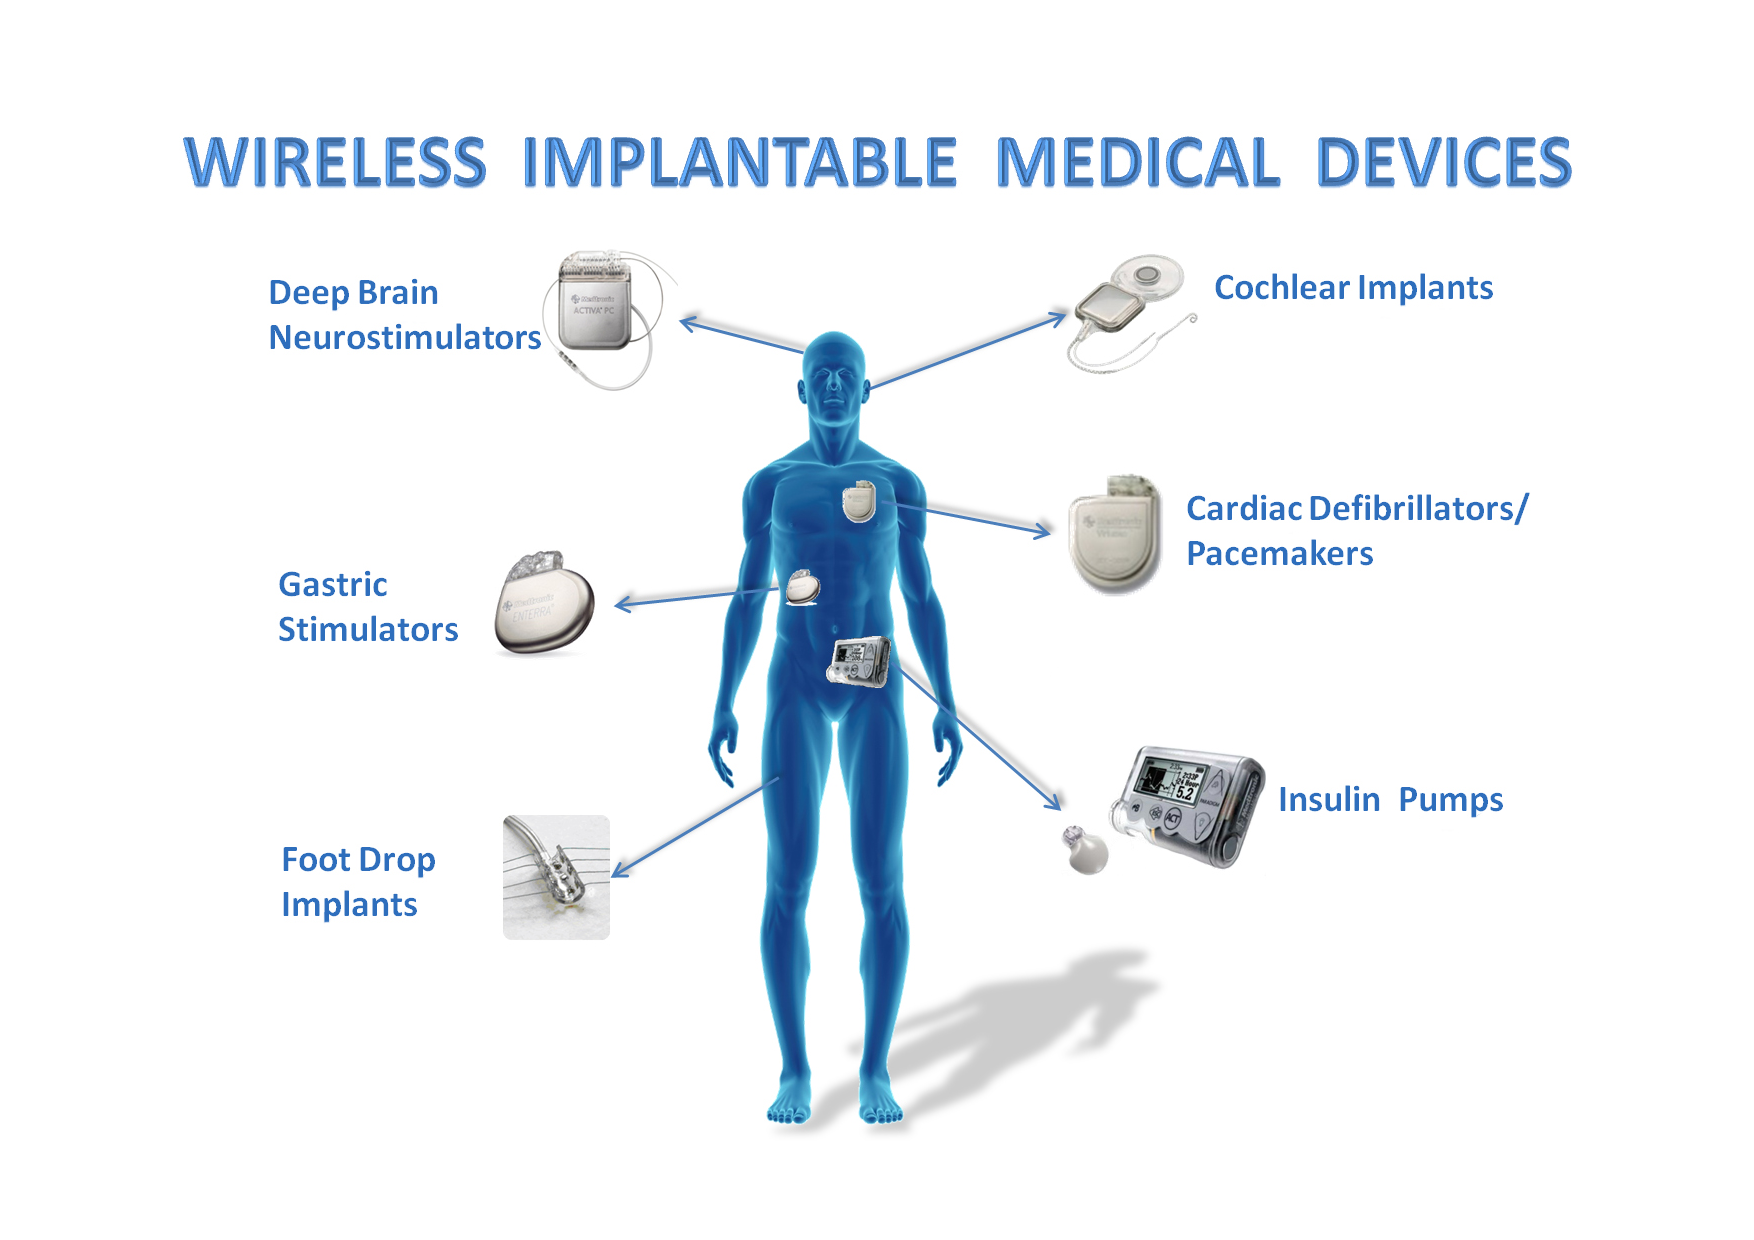
\includegraphics[width=8.5cm]{wmd}
\caption{Wireless Medical Devices \cite{wirelessmd}}
\label{fig_one}
\end{figure}

Then we went to the doctor who prescribed either medication or took us to a radiologist to find out more about our state of health in a \ac{MRT}. Maybe we had surgery and during the intervention a \ac{CT} gave further information about the intervention to the surgeon. 
Medical devices and machines affect our everyday life which makes hackers getting interested in those devices. As a consequence, there already occured several attacks on hospital systems and medical devices because of their non-protected and easy-encrypted access points or insecure interfaces.

\subsection{Medical Telediagnosis}  \label{telediagnosis}

Telecommunication technologies are often used to provide medical information and services such as remote and flexible surgery (see \ref{fig_two}). The process by which electronic, visual and audio communications are used to support practitioners at remote sites with diagnosis and consultation procedures is called medical telediagnosis \cite{telediagnosis}. To give an example of the procedures, telediagnosis are used in remote clinical examinations or medical image transfers. Furthermore, there exist various laws and constraints regarding the access of data contained in 'Personal Medical Files'. These laws depend on the particular country and the local health care system. Generally, requirements and communication standards for the information exchange in medical systems are specified by international entities, such as \ac{IHE}. Nevertheless, when using telemedicine applications, some countries require a certification to allow their deployment. In the following, six important requirements to telemedicine devices will be explained in detail.

%figure 2
 \begin{figure}[!ht]
\centering
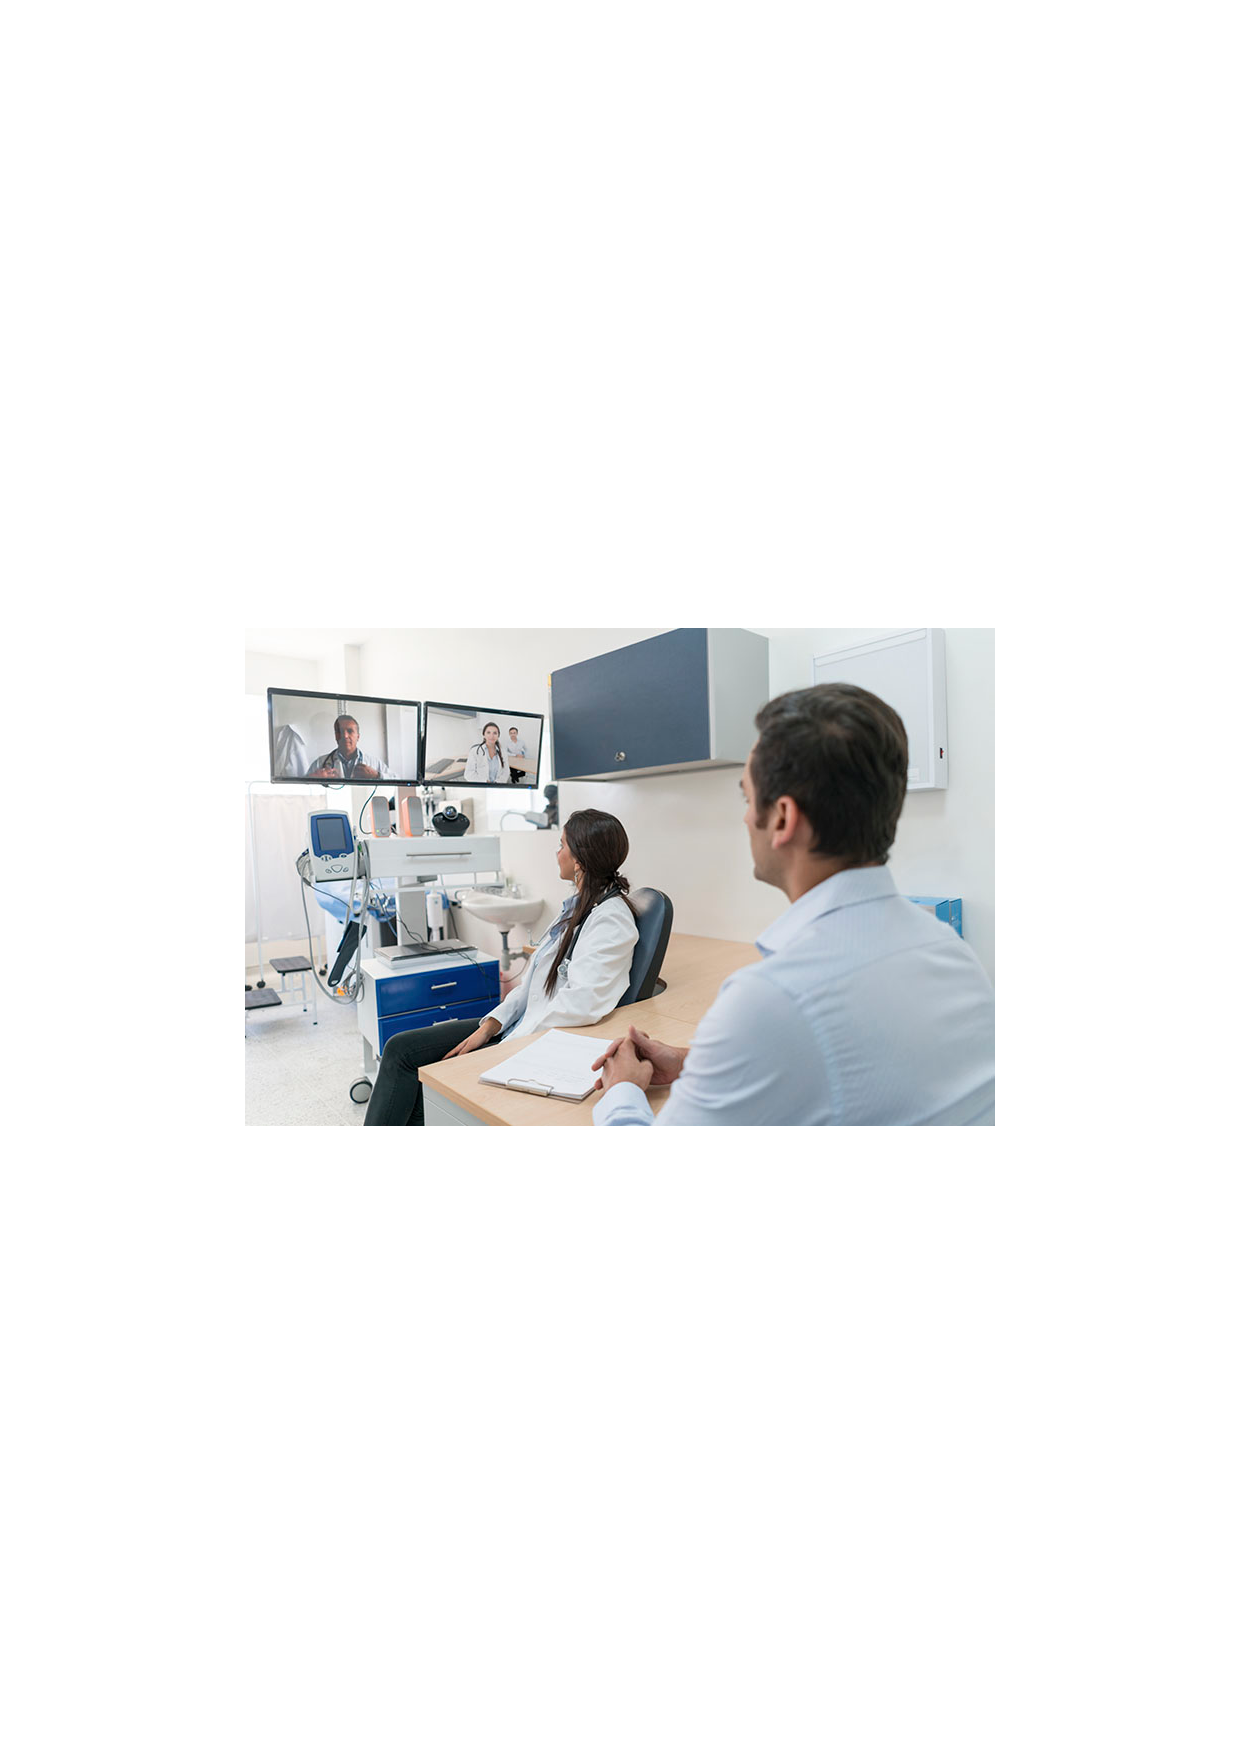
\includegraphics[width=8.5cm]{telemedicine}
\caption{Telemedicine conference \cite{telemed_bild}}
\label{fig_two}
\end{figure}

First of all, the authentication is very important for both the running system and the computer or hardware. In every information system, there should be an access control which asks for the users' authentication data so that only specific users will be verified. Moreover, computers need to be authenticated in different applications, in such a way as only allowed computers can connect to an application. Besides it should be clear who is allowed and authorized to use the system. If the user is not allowed to use the system, he cannot perform transfer within it. In the past few years, there have been established several authentication technologies, such as \ac{RFID} cards or biometrics.
According to J.-B. Aupet et al. \cite{telediagnosis}, it is highly recommended to use an unique mean of authentication (e.g. RFID) and a \ac{LDAP} repository to store user logins and passwords. Alternatively, \ac{SSO} systems can be used in order to ask the login and password once and to use it for each application. At this point, the one should not forget the possibility of password attacks and the misuse of the SSO systems by third parties.

Secondly, the data in telemedicine applications should be transfered and stored securely. As a 'standard' for secure network connections, \ac{VPN} has been established and used. The user who accesses the network (e.g. WLAN or LAN of hospital) via a VPN gateway creates a secure and private connection to the external network. In addition to that, the information he sends through VPN should be encrypted, for instance with \ac{DES}, \ac{3DES}, \ac{AES} etc.). Furthermore, the data should be transfered using a \ac{SSL} or \ac{TSL}, a hybrid encryption protocol for a secure data transfer through the internet. 

Besides secure transfer protocols and connections, the integrity should be controlled through digital signatures. The development of digital signatures has been highly improved in the last five years but is not optimized yet. For example, there exist Tablets and Smartphones which make it possible to write on them, to store the digital handwritten text internally and to share the file with other devices. But the algorithms which detect a specific handwriting or signature from a specific doctor are not precisely yet. Nevertheless, digital signature would speed up the referral and prescription process very much.
 
Thirdly, telemedicine applications should offer audit trail tools which track all exchanges of medical data. As a standard way to log events, IHE \ac{ATNA} has been established (see \ref{fig_three}). \ref{fig_three} shows the IHE ATNA profile which specifies security requirements to all systems communicating within the same network. The data exchange between the systems is based on \ac{XDS.b}, a standardized security infrastructure. In the right corner in \ref{fig_three}, there is a blue 'Audit Repository' which contains information about the storage of all Audit informations in the network \cite{ihe_atna_bild}. Furthermore, \ref{fig_three} shows the bidirectional, certificate-based authentification of the communicating systems and enables the encryption of transport. Referred to ATNA, the affected systems authenticate all users and for the across system authentication, there exists a reference to other IHE profiles. In the top bottom corner of \ref{fig_three}, there is a red marked 'Secure Node grouped with Any IHE Actor' which enables the connection to other IHE profiles. Additionally, events and audit trail messages should be based on \ac{DICOM}, \ac{HL7}, \ac{ASTM} standards. 
 
 %figure 3
\begin{figure}[!ht]
\centering
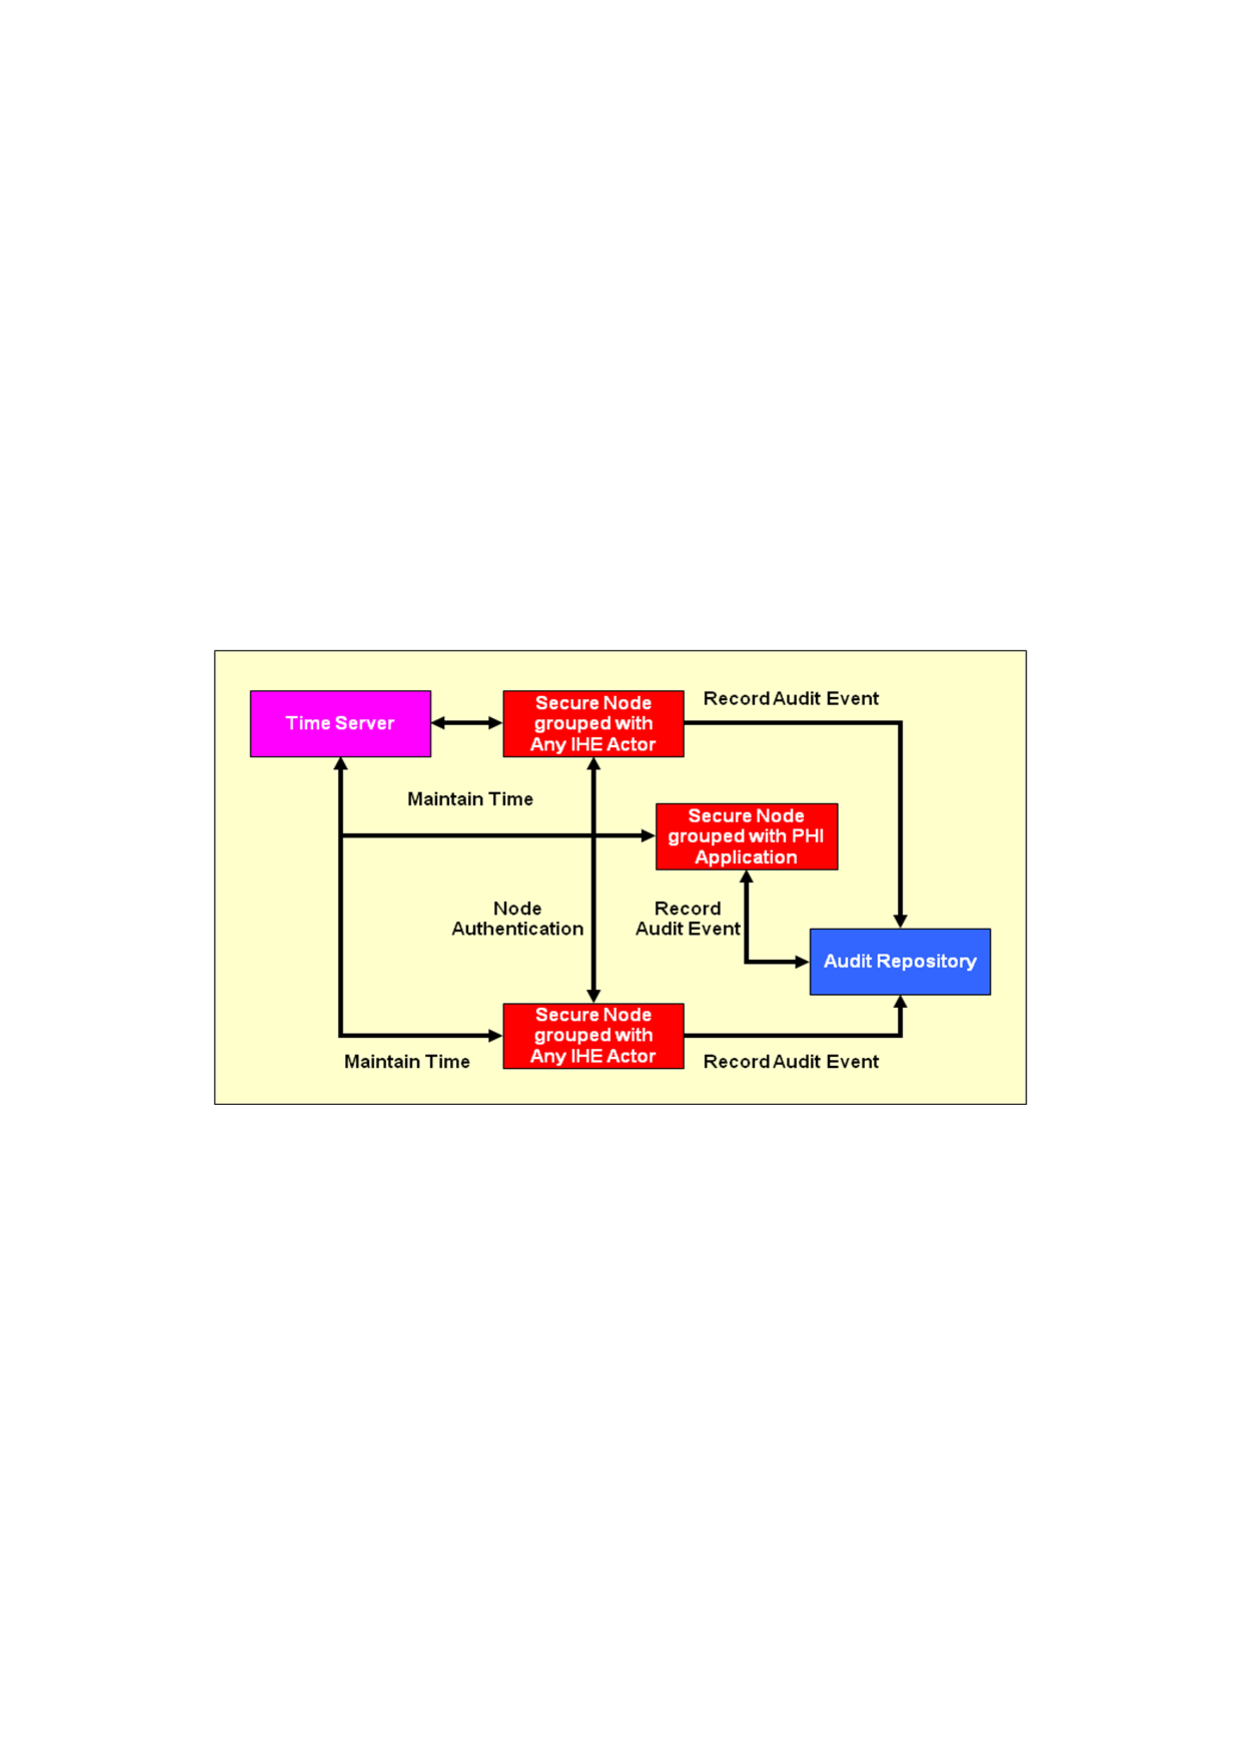
\includegraphics[width=8.5cm]{ihe_atna}
\caption{IHE ATNA audit trail process \cite{ihe_atna_bild}}
\label{fig_three}
\end{figure}

\ref{fig_four} gives an example of the functionality of the IHE XDS.b standard. All participated actors are coloured. In the top corner there is the personalized 'Patient Identity Source' which is stored in the 'Document Registry' in the center of \ref{fig_four}. In the bottom left corner the 'Integrated Document Source/Repository', which contains the 'Document Source' and 'Document Repository', is pictured. If a clinician (e.g. a doctor or nurse) wants to see or edit the patient's data, he can set a 'Registry Stored Query' which accesses the 'Document Registry'. As an answer the XDS.b standard will respond with the corresponding 'Document Set'.

%figure 4
\begin{figure}[!ht]
\centering
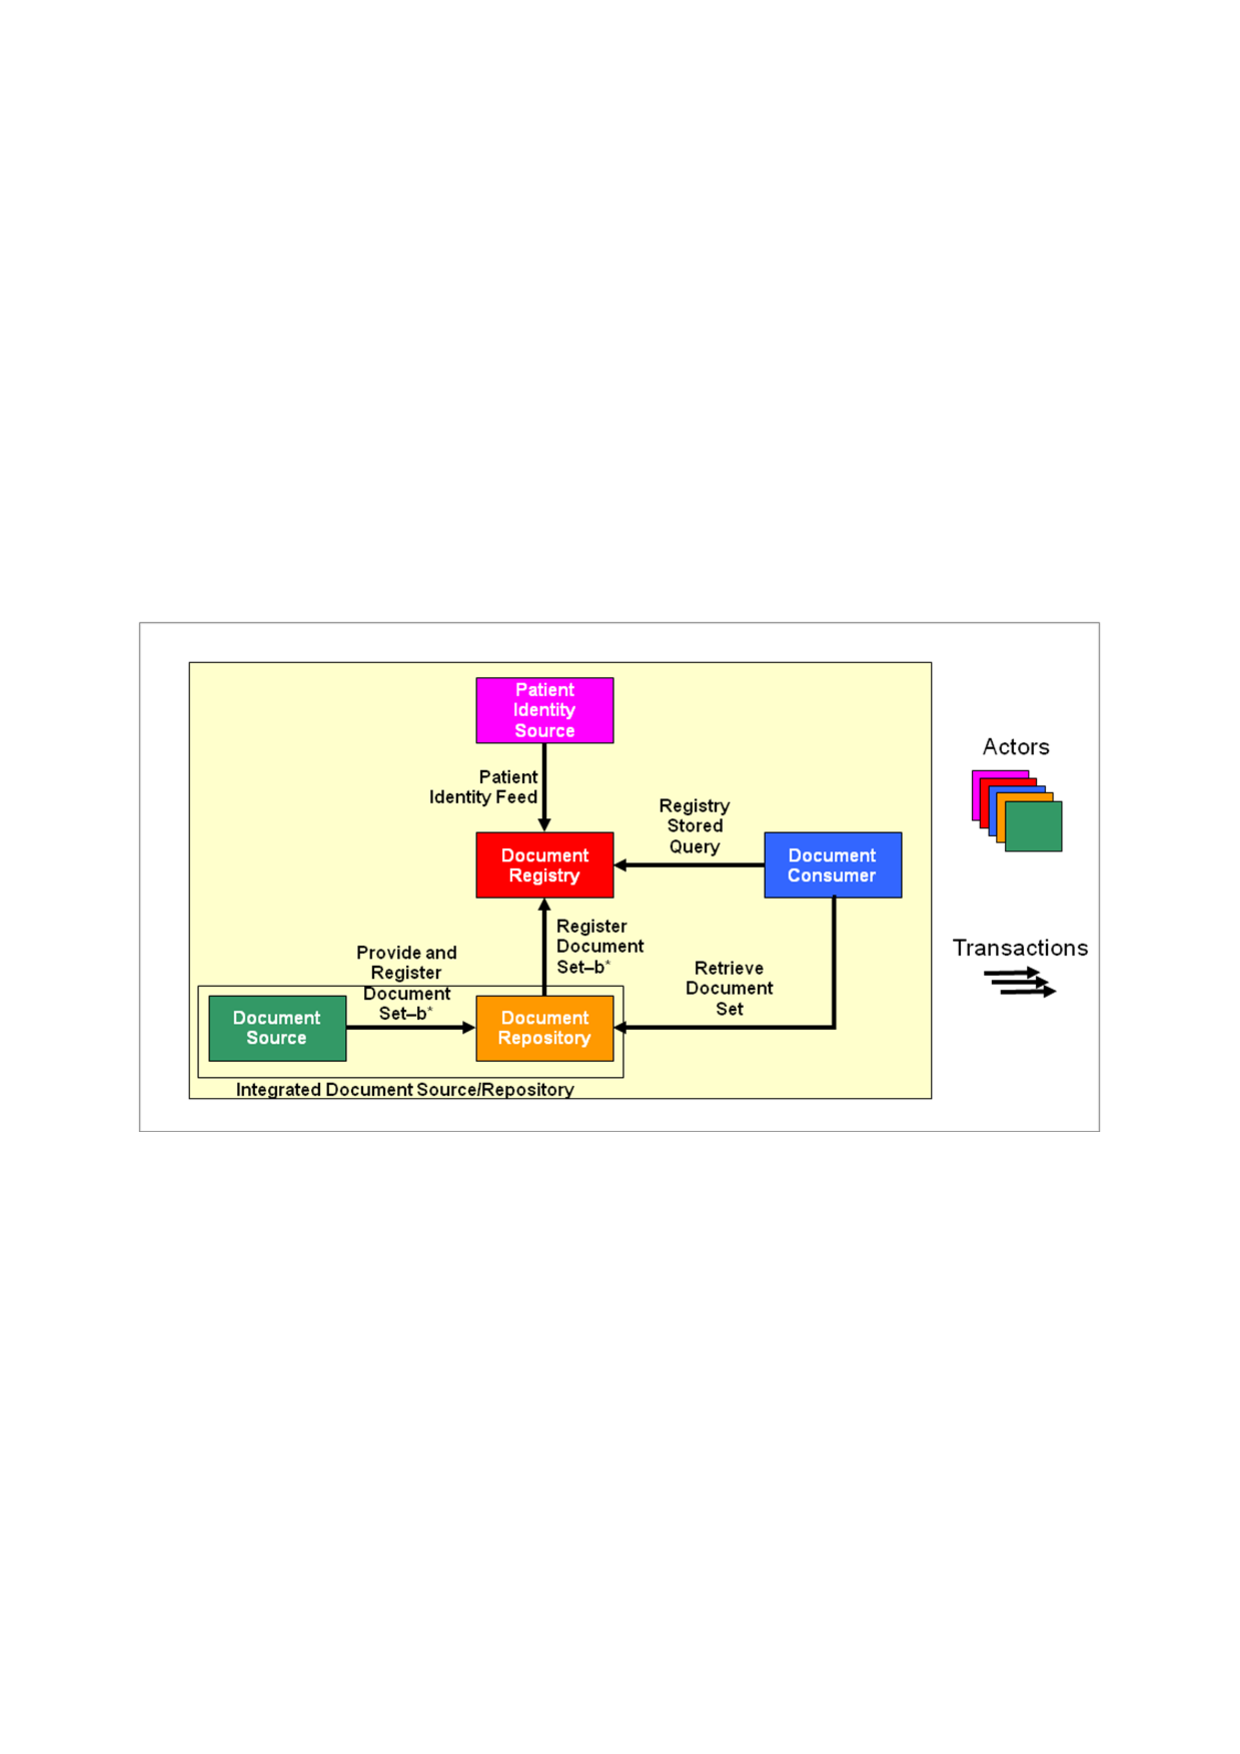
\includegraphics[width=8.5cm]{IHE_cookbook_xds}
\caption{IHE XDS.b  \cite{ihe_xds}}
\label{fig_four}
\end{figure}

On top of that, to ensure a secure data transfer, patients' informations should be identified exactly and only once for each patient. To identify a particular patient and to ensure that one patient is highly identified, the \ac{PIX} standard, established from IHE, should be used. The PIX Integration Profile supports the cross-referencing of patient identifiers from multiple Patient Identifier Domains. 
\ref{fig_five} gives an overview of the 'Patient Identifier Cross-reference Domain'. In the top left corner of \ref{fig_five}, there is the 'Patient Identifier Domain C', which transmits 'Patient Identity Feed' and 'Patient Identity References' to the 'Patient Identifier Cross-reference Manager'. In the top center of \ref{fig_five}, the 'Patient Identifier Cross-reference Manager' coordinates two 'Patient Identifier Domain', which send 'Patient Identity Feed' and get the associated  'Patient Identity Cross Reference'. These 'Patient Identity Cross References' are consumed by the 'Patient Identifier Cross-reference Consumer'. Each 'Patient Identifier Domain' is connected to other 'IHE Actors'. The connection to these actors is realized by 'Internal Domain transactions'. In general, the PIX Integration Profile supports two domains which differ in their size. There can be either a single system or a set of interconnected systems that all share a common identification scheme \cite{pix}.

%figure 5
\begin{figure}[!ht]
\centering
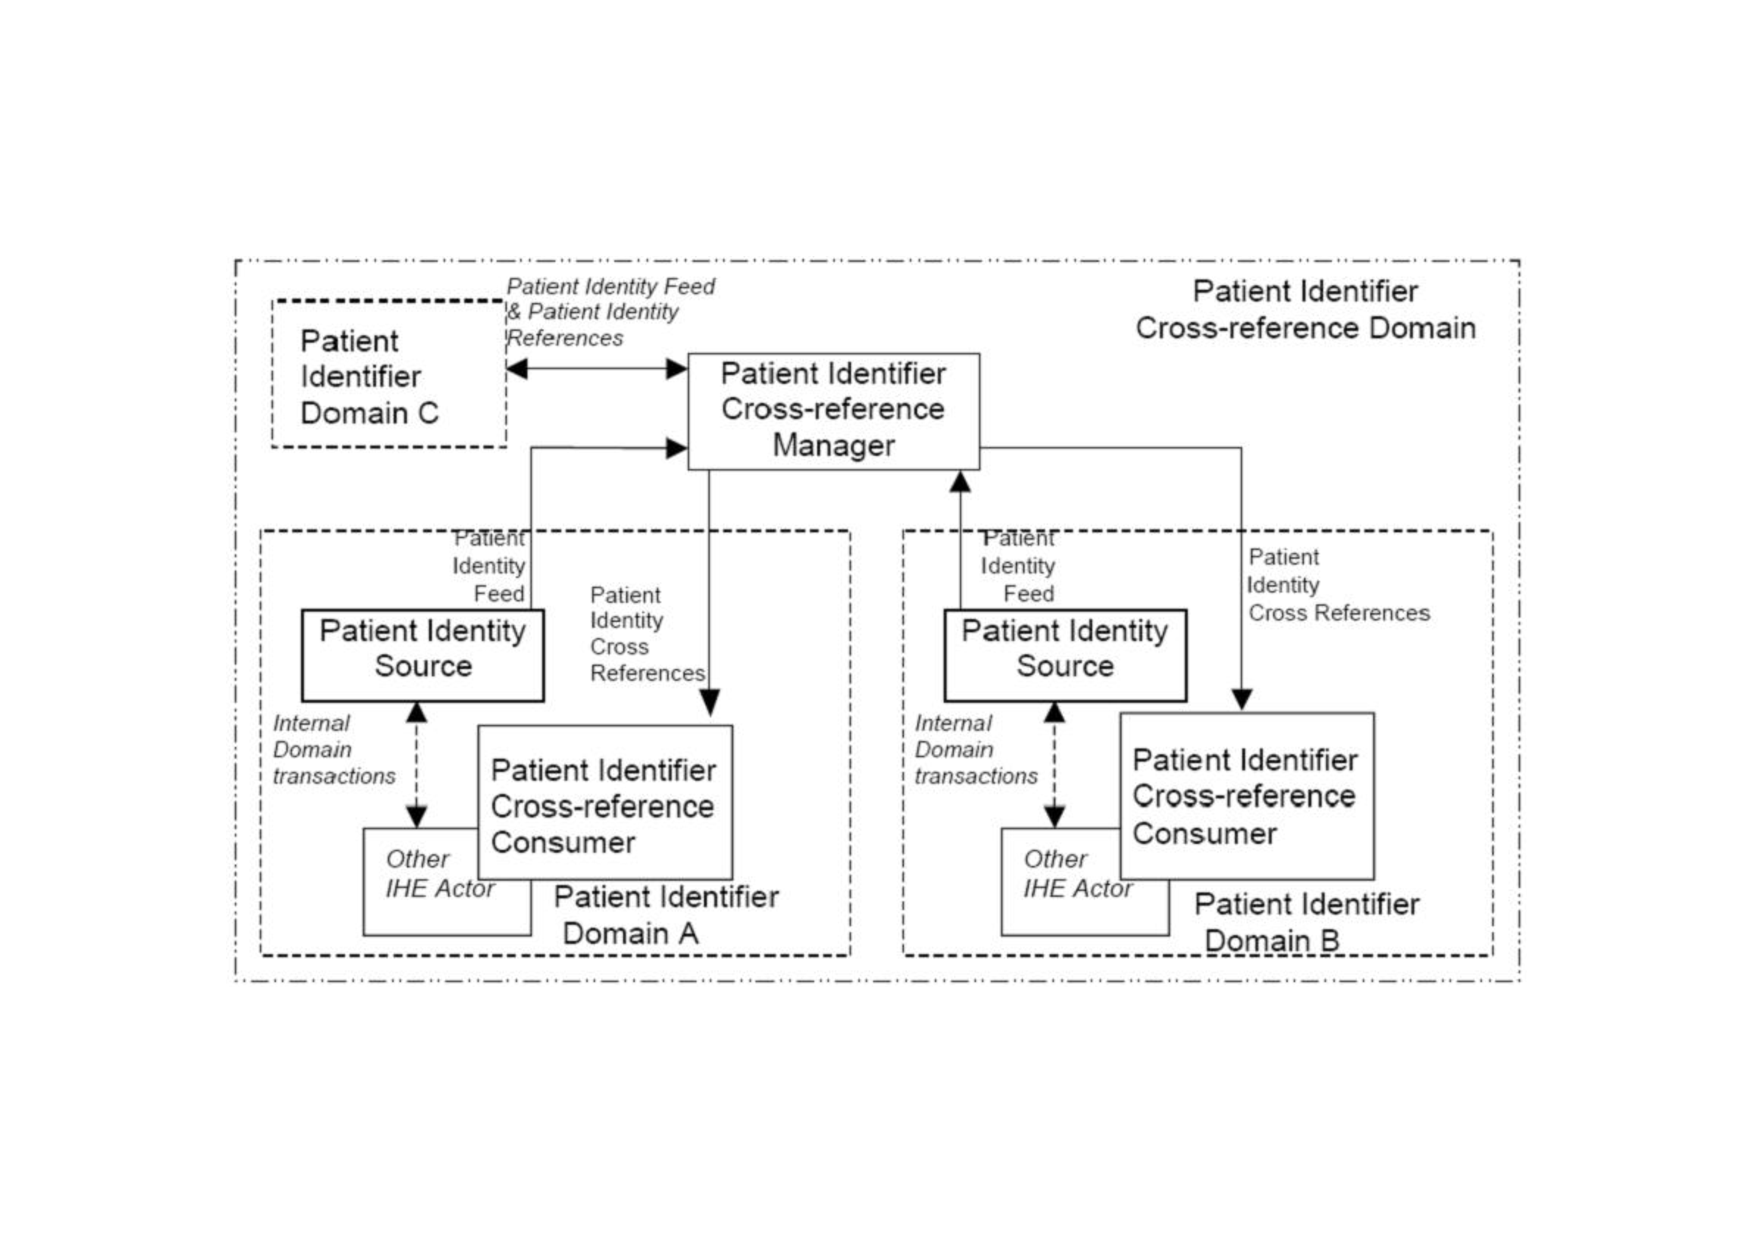
\includegraphics[width=8.5cm]{PIX}
\caption{IHE \ac{PIX} standard  \cite{pix}}
\label{fig_five}
\end{figure}

Another important requirement is the storage of personal, sensitive data. J.-B. Aupet et al. \cite{telediagnosis} recommend two ways of storing personal patient's data. On the one hand, to protect data from intrusion, it should be encrypted and put on protected servers. On the other hand, to protect data from loss, servers should be replicated with backup functions using the specific life cycle of data. Recent data is stored on server hard disks and later on other types of supports according to their age.

Last but not least, the bandwith of telecommunication networks is important for every application. Depending on the particular country, the health care system runs on a separate network. This implies that applications which should be deployed on the network, need a certification. With this certification, the software is tested for bandwith consumption. Thus, deploying an application which could breakdown the network can be avoided by denying the permission to run the application. 


\section{Typical weak points in medical setting} \label{weak points}

\subsection{Historical inflection points}

In the past 30 years there have been several incidents in hospitals and their local system architectures. Especially medical devices had been of great interest to hackers. In the following, the past events of cyber threats and other attacks on medical devices will be explained.

According to Burns et al. \cite{burns}, there have been four inflection points on medical devices. 
In the years from 1985 to 2000 (first period) especially broader, complex systems in hospitals had been attacked by unauthorized people which produced disasters. 

In the 2000’s (second period), there had been an increase of implantable medical devices, such as implantable cardiac defibrillators. 2005 a 21 years old cardiac patient died from an attack on his implant which manipulated the regular heart rate. As a consequence the \ac{HCMSS} developed a roadmap for overcoming crucial incidents and challenges concerncing the design, manufacture, certification and use of medical device security.    
 
The third period, with the major threat of unauthorized access to devices that could cause harm took place in the years from 2006 until now. In the year 2006, the amount of attacked hospital systems increased because of software updates which offered an interface for hackers. 2011 there were executed peer-reviewed defenses against unauthorized access to implantable medical devices. So called 'Radio Frequency Shields' had been used for acting as a proxy for communications with implantable medical devices. These proxies actively prevented any device other than itself from communicating with the implantable mobile device by jamming all other communications.  
 
The forth and last period (2012 until now) includes remote threats to medical device security. The cause of this impact were the manufacturing of medical devices which were able to connect directly (but also indirectly) to the Internet/network (\ac{LAN}/\ac{WLAN}). On the one hand, the devices allowed the real-time monitoring of patients and improved the software management (e.g. remote installation of software updates). But on the other hand, cybersecurity threats had become prevalent in the network age so that the protection of medical devices is more critical than of other device types.  
  
As an answer to this problem a \ac{FDA} draft guidance for the management of cybersecurity in medical devices had been published in June, 2013. The draft deals with the identification of assets, threats and vulnerabilities. Furthermore it deals with the assessment of the impact of threats on device functionality, users or patients. Moreover, the draft includes the assessment of the likelihood of a threat and of a vulnerability being exploited as well as the determination of risk levels and mitigation strategies. It claims the assessment of residual risk and risk acceptances criteria. Not only the \ac{FDA} published a solution against cyber threats, also the \ac{NIST} received so called 'Trust challenges' (2013-2016), including hardware failures, software errors, radio attacks, malware and vulnerability exploits and side-channel attacks.
To remark further incidents in the healthcaring sector, the next two sections will give examples of currently occuring security problems in the USA \ref{USA} as well as in Germany \ref{GER}.

\subsection{USA} \label{USA}

When we go back to the year 2013, the US Government took notice on a project called  \ac{ThaW} against threats on medical devices \cite{burns}. This project was founded by the \ac{NSF} with the goal 'to authenticate clinical staff to tablet computers' \cite{burns} and 'to provide patients a usable way to control the information that mobile sensors collect about them' \cite{burns}. But why did the government took notice of the vulnerability so lately? To understand the problem of security beyond devices which collect medical data, we should take a look at the 'Therac-25' (a radiation accelerator, see \ref{fig_six}) which had caused lots of harm to the patients.

 %figure 6
\begin{figure}[!ht]
\centering
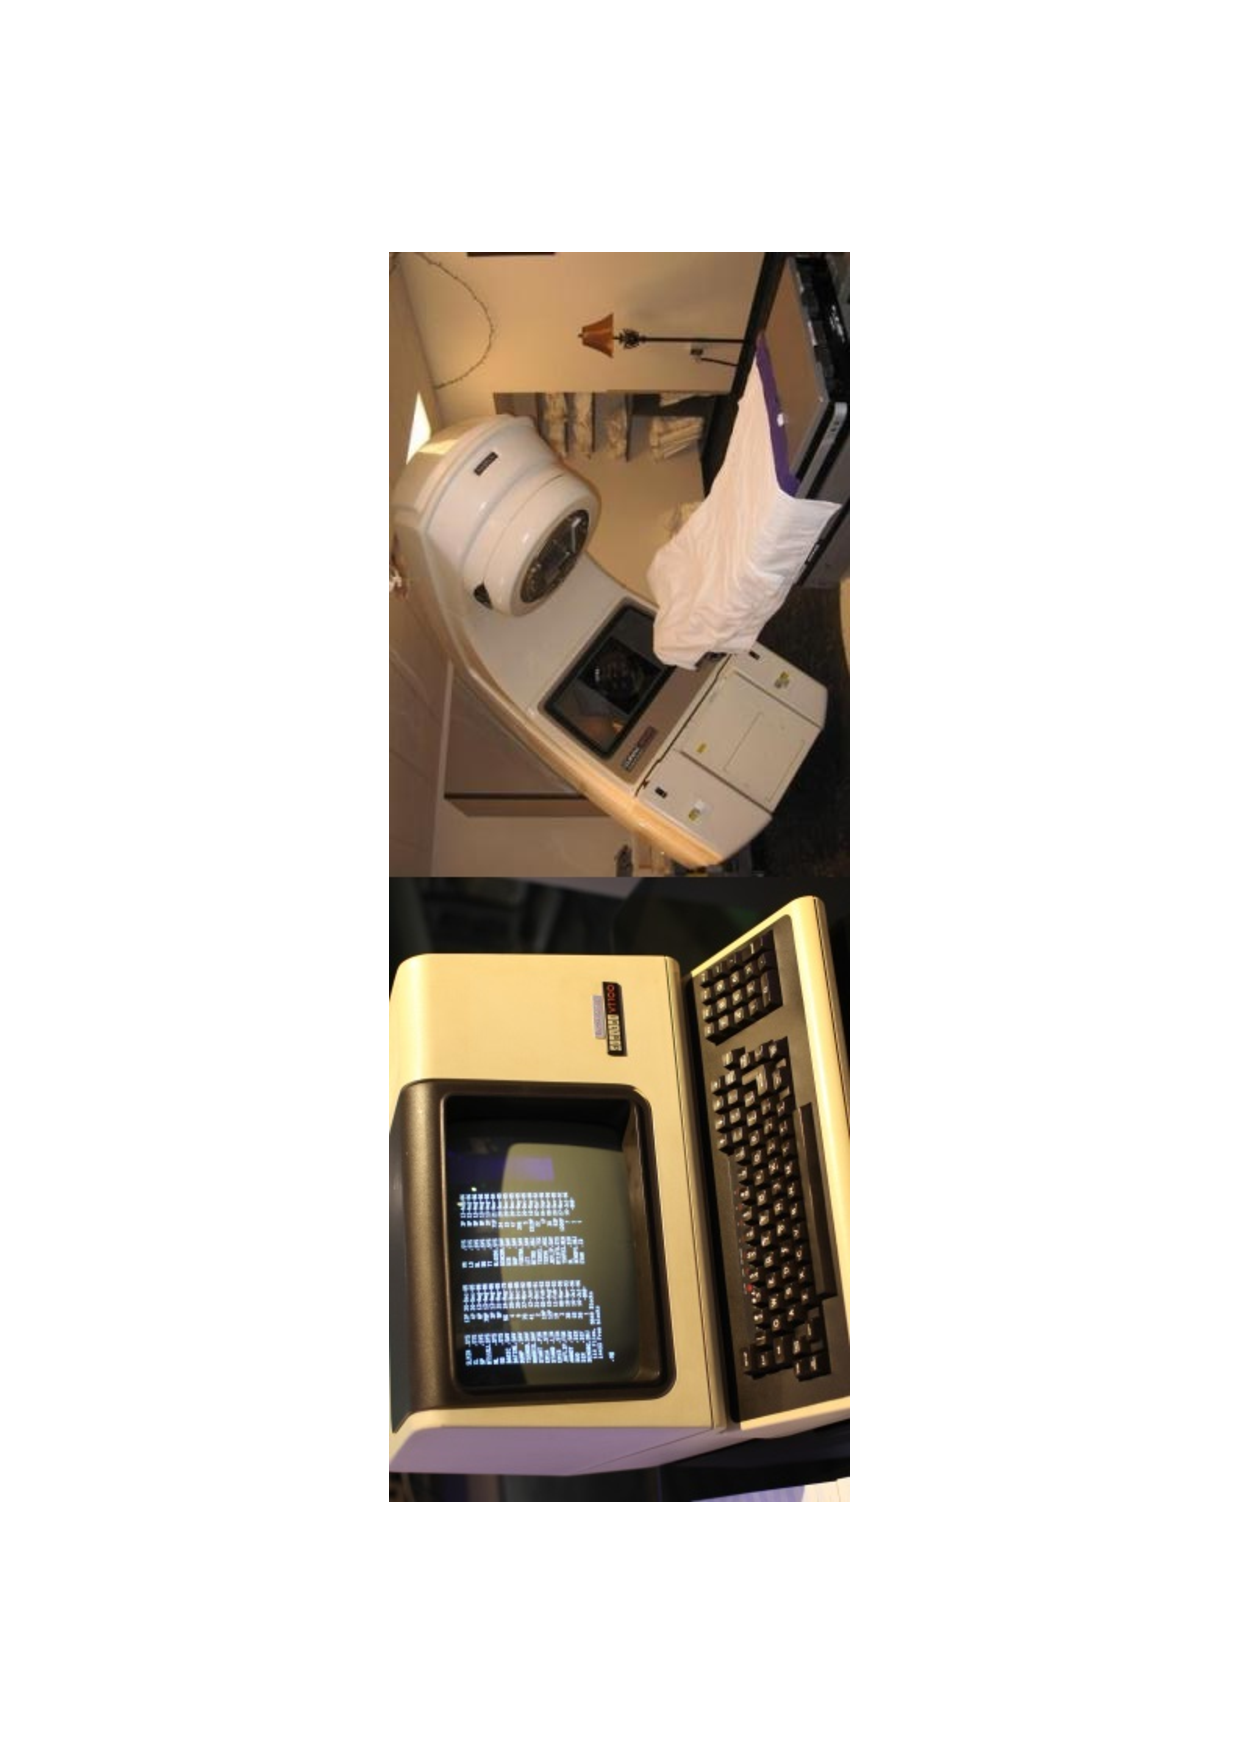
\includegraphics[height=8.5cm, angle=-90]{therac25}
\caption{Therac-25 radiation accelerator \cite{therac_bild}}
\label{fig_six}
\end{figure}

From June 1985 to January 1987, the 'Therac-25' had been used for patients suffering from tumors. But there were some differences between the 'Therac-25' and its previous models. With the new radiation accelerator it was possible to regulate the intensity of radiation from outside the treatment room. As a consequence of the user errors, faulty software engineering and insufficient training support six people died.
But the 'Therac-25' was only the beginning of the software failure in hospital systems and medical device programs. Actually, hospitals consider primarily treating people and helping to improve their health than thinking about security. In fact, many other institutions (e.g. financial services) cared about security earlier than health care institutions.
In the year 2002, there was a \ac{BIDMC} network failure triggered by researchers who flooded the network with data. The impact caused delays in access to critical information and IT-systems and deteriorated the network diagnoses. After that happened, the principal point of failure was declared as a software program for directing traffic on the network. The program was overwhelmed by a combination of data volume and network complexity that exceeded the software specifications. Thus, security problems cannot only be triggered by unauthorized access but also by violation of the product’s specifications. 

\subsection{Germany} \label{GER}

In the year 2015 several tomographs (Positron Emission Tomography and Single-Photon-Emissions-Tomography) from Siemens had been in use in german hospitals \cite{sicherheitsiemens}. At that time it was already known that the tomographs had security vulnerabilities such as they were easy to hack from outside the network. One reason for that vulnerability was the operation system under which the tomography had been running. As the US agency \ac{ICS-CERT} has published that there had been security holes in tomographs from Siemens they also mentioned that one of the main risks is Windows 7. Furthermore there were ready-made exploits which can be used without any expert knowledge. As a consequence, attackers can “speak” over the network with the devices by accessing the network of the hospital. As a solution, Siemens announced 'security updates' available for all affected tomographs, only as a brief security note \cite{siemens}. Actually, the date (until which day) the patches would be available for users had not been published yet. 

In March 2017 there was an incident in several hospitals in Germany, triggered by a disinfection system made by Miele (see \ref{fig_seven}). It was related to the IT consultant Jens Regel who had found out that there was a vulnerability in terms of a 'web server directory traversal bridge'. That bridge made it possible for any person to contact the system with a simple 'telnet' command and to get access to all data from the machine and the passwords. After he had found that leak in the disinfection system, he tried to call Miele but did not get any answer (even after several months). As a consequence, he published his problem on the website 'Full Disclosure Mailing List' \cite{mailinglist} and got response after a few days. Even the company itself (Miele) reacted to the problem and asserted that there had been a breakdown of communication. Furthermore, Miele promised to release security updates in the near future and assured that it should not bring any complications or danger to the affected models because they had no \ac{WLAN} interface. Even though the affected disinfection systems have ethernet interfaces to be connected to printers or barcode scanners in the hospital. Hence, through those interfaces it could be possible for attackers to get access to further unsecured machines in the hospital once they were in the internal network.

% Grafik in einer 7
\begin{figure}[!ht]
\centering
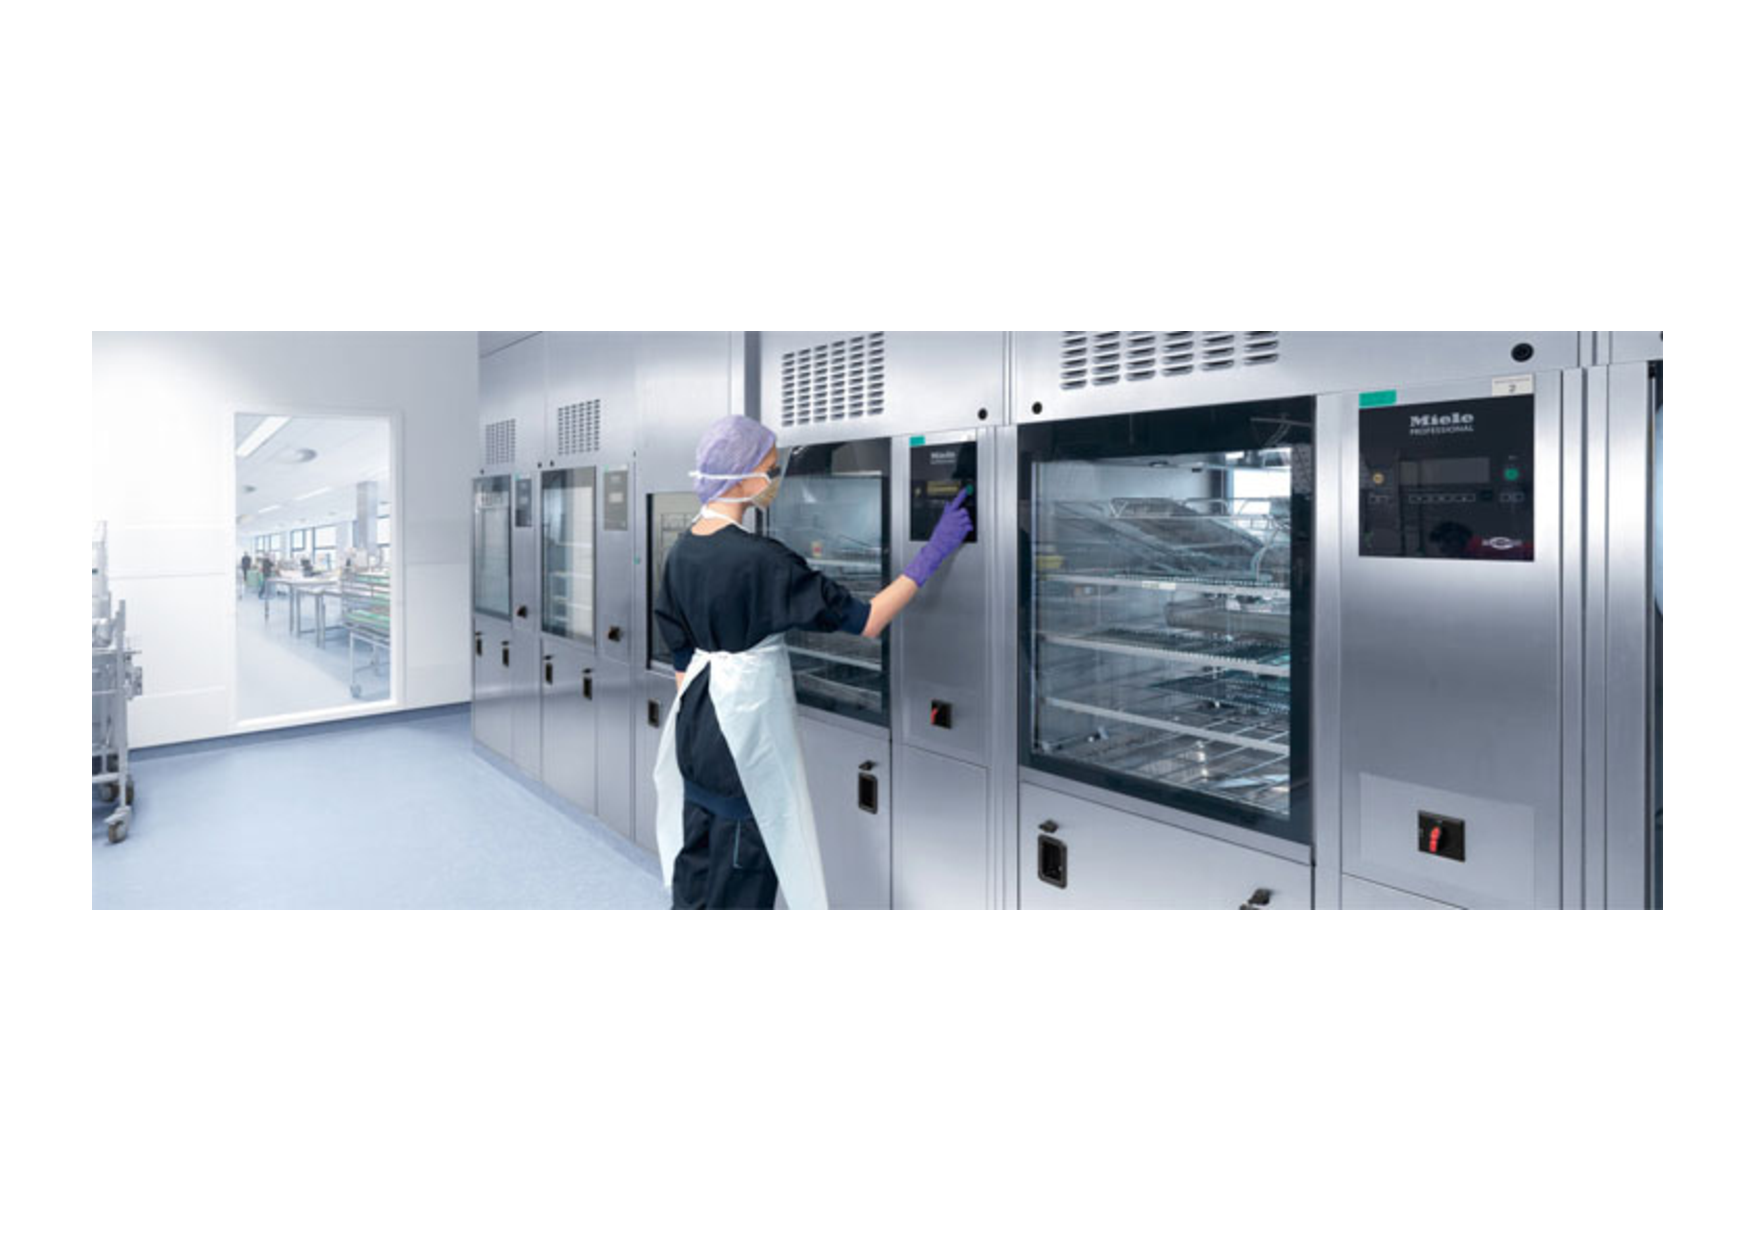
\includegraphics[width=8.5cm]{pg8528}
\caption{Miele disinfection system (Model No. PG8528) \cite{pg8528} }
\label{fig_seven}
\end{figure}

Not only large system landscapes in hospitals are threatened by attackers but also small medical devices, such as implants which are of great interest to the attackers. In August 2017, the corporation MedSec \cite{medsec} (which is specialized on testing medical devices and their security) detected a big vulnerability at cardiac pacemakers made by Abbott (see \ref{fig_eight}, \cite{herzschrittmacher}). At that date it was possible to manipulate the pacemakers via radiocommunication and to intercept the communication between the pacemaker and the programming machine. A very critical fact was that the affected pacemakers from Abbott did not have any authentication mechanism. Consequently, it was possible to get access to the implants and to perform configuration changes and execute remote commands. Abbott reacted to the detected security issue with the note that all pacemakers (see \ref{fig_eight}), which had been produced since 28 August 2017 do have firmware updates. But if patients had older cardiac pacemakers, they have to go to the doctor who will run the updates by laying a machine on their body near to the pacemaker. After three minutes, the patch should be done and during the update, the pacemaker runs in "backup-mode" which means that it provides the patient's heart with the needed impulses.  

%figure 8
\begin{figure}[!ht]
\centering
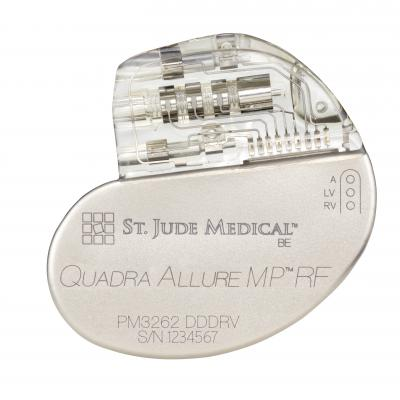
\includegraphics[width=8.5cm]{pacemaker_abbott}
\caption{Abbott (earlier: St.Jude Medical) Assurity MRI \cite{herzschrittmacher} }
\label{fig_eight}
\end{figure}

Besides the authentication leak, pacemakers already had security issues in the past. For example, in 2008 cardiac pacemakers were accessible from outside through their proprietary radiocommunication interface. At that time, attackers had used the access to those implants for reading the data and programming the pacemaker. At this point, we should not forget, that pacemakers are only available from small distances (0.5-0.9 m) which makes it more difficult in case of an attack.
In the year 2013, Barnaby Jack, who firstly discovered security holes in banking systems and later manipulated medical devices, should present his new results at the 'Black Hat' conference in Las Vegas ( \cite{herzschrittmacher}). His talk should include the solution how to hack implantable medical technology from large distances. Unfortunately, he died of an unknown cause of death one week before the conference. 

\subsection{Points of attack}

As already mentioned, there are several points of attack on medical devices, such as drug infusion pumps, linear accelerators or pacemakers. One new risk are devices with \ac{NFC} or WLAN interfaces because they are vulnerable to external attacks which use the devices' bugs and leaks. Generally, medical devices can be divided into two big groups: \ac{IMD}s (see \ref{fig_nine}) and \ac{BAN}s (see \ref{fig_ten}). 
\ac{IMD}s include medical devices which are embedded inside the human body. They make it possible to continuously and automatically manage health conditions, e.g. cardiac arrythmia or Parkinson's disease. \ac{IMD}s had become pervasive because of the increasing energy efficiency and low costs of embedded systems. Thus, they made it possible to provide real-time monitoring and treatment of patients (e.g. insulin pumps). As one can see, \ref{fig_nine} represents a possible network of implantable medical devices. On the left side there is drawn a patient with various implants. Those \ac{IMD}s are connected with the software through a magnetic field. Particularly, the magnetic field can be used for data exchange and communication between the implants and the programm. For each call the field will trigger a magnetic switch. The users (doctors) can send commands or requests from the program to the implants and each implant can answer with telemetry signals.

%figure 9
\begin{figure}[!ht]
\centering
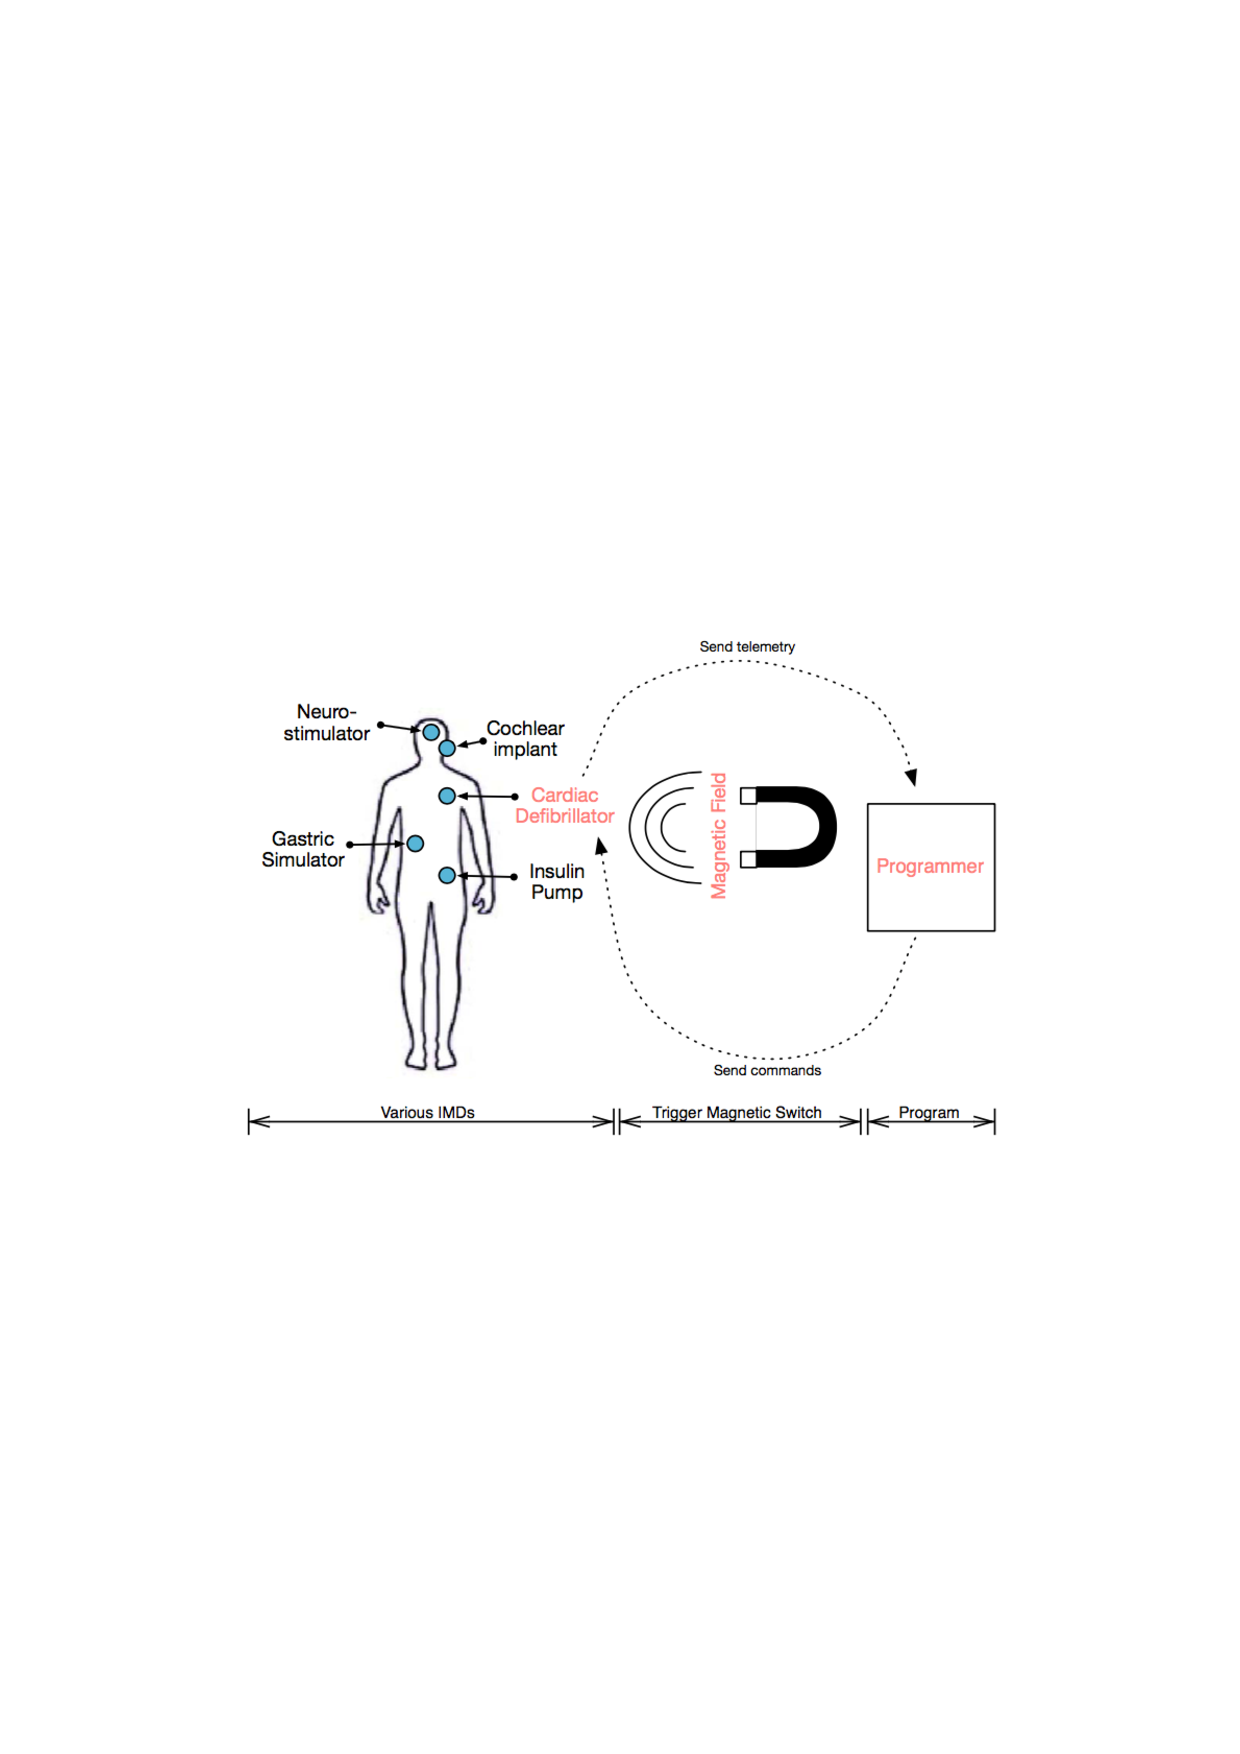
\includegraphics[width=8.5cm]{imd_icd}
\caption{Implantable Medical Device Network \cite{securityprivacy}}
\label{fig_nine}
\end{figure}

\ac{BAN}s can be seen as wireless networks of wearable computing devices which enable remote monitoring of a patient's health status. Through the network, sensors collect a range of physiological values (e.g. heart rate, blood pressure, oxygen saturation, temperature) and provide the appropriate actuation and treatment (for example to regulate the heart rate or halt tremors). Furthermore, there exist on-board radios which enable wireless data transfer and medical telemetry for monitoring and configuration without sacrificing the patient's mobility \cite{securityprivacy}. \ref{fig_ten} shows a possible scenario. The functionality of \ac{BAN}s can be divided into three steps. The first step includes the sensors, measuring and collecting all data they get from the patient. After that, a 'sink' collects all the detected data and sends it forward to the network which is drawn as a cloud in the center of \ref{fig_ten}. Lastly, the forward-sended data will be collected and provided for the remote caring sector, symbolized as a red cross.

%figure 10
\begin{figure}[!ht]
\centering
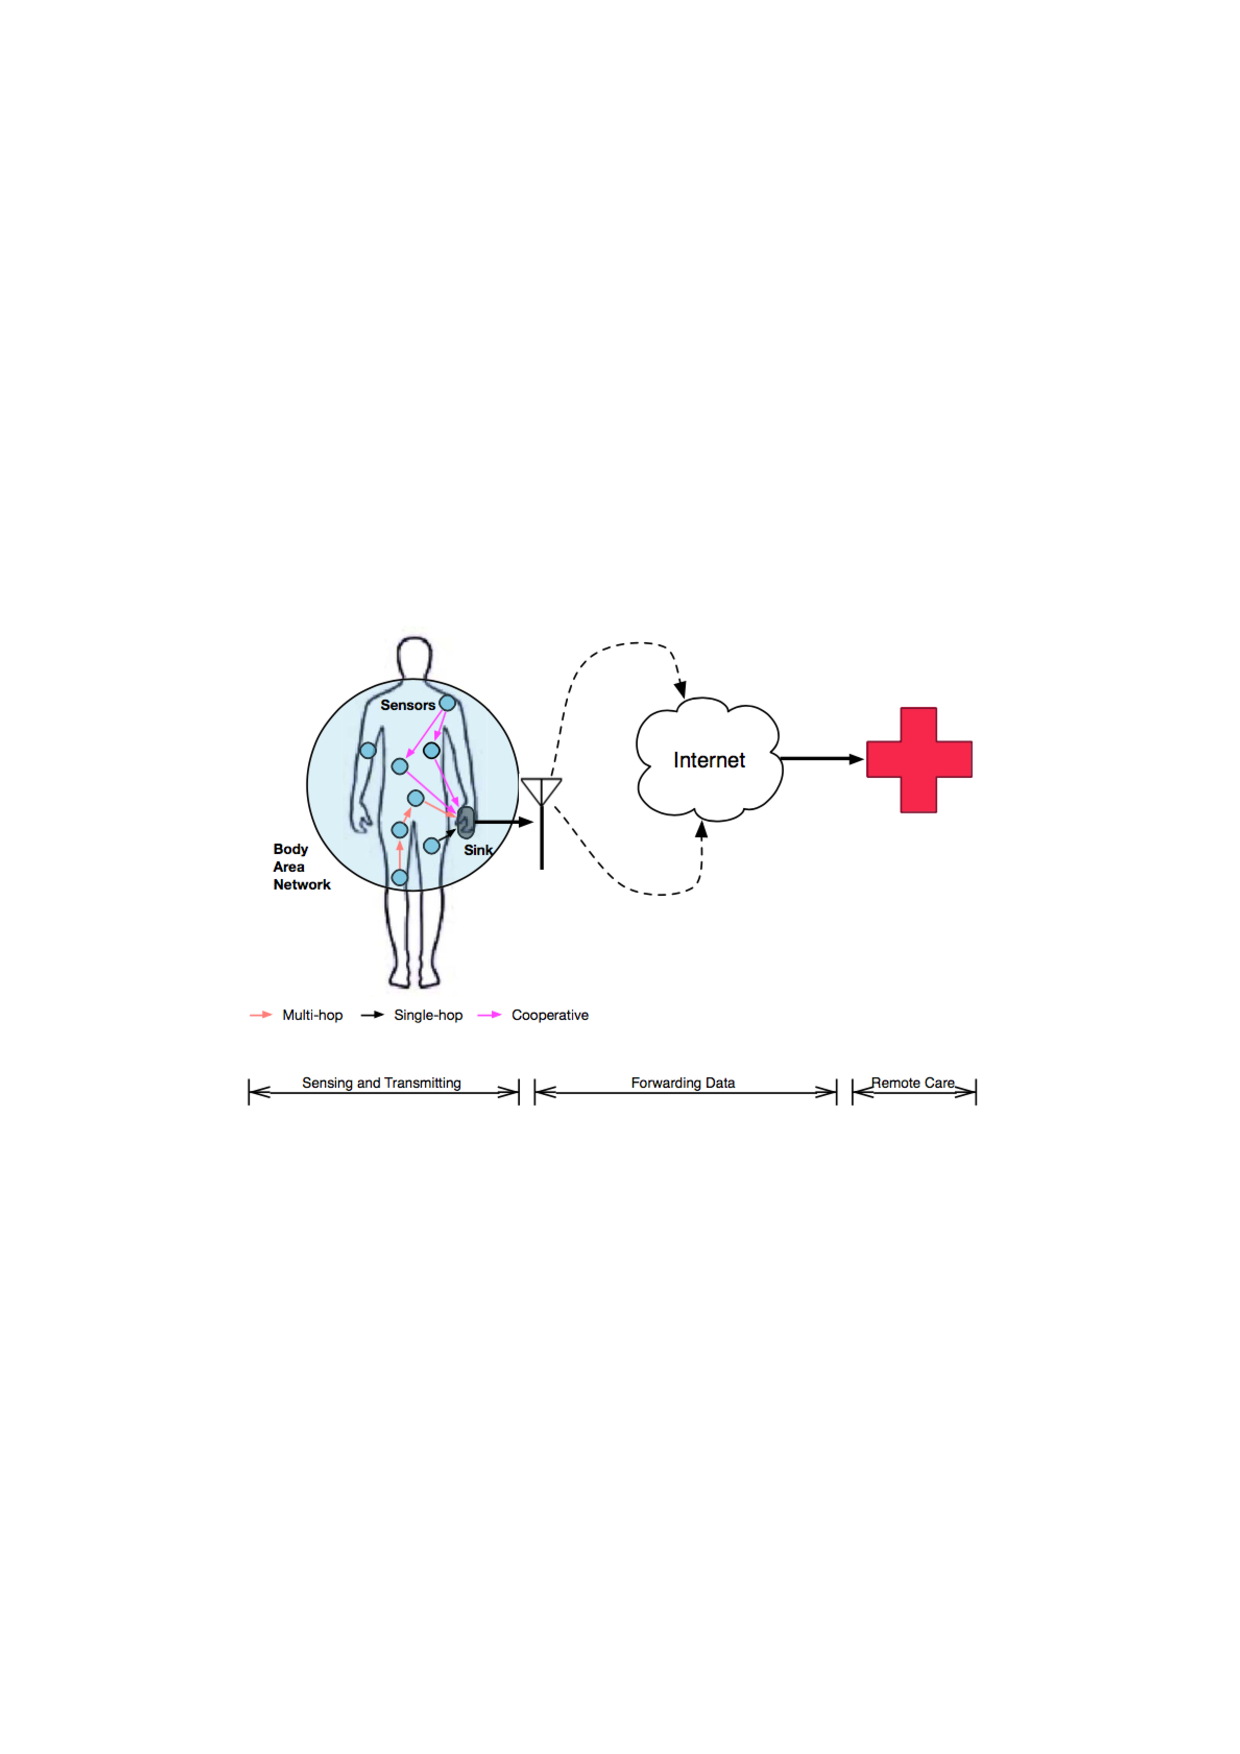
\includegraphics[width=8.5cm]{BAN_architecture}
\caption{Body Area Network \cite{securityprivacy}}
\label{fig_ten}
\end{figure}

\section{Countermeasures} \label{counter}
\subsection{General countermeasures}

As explained in the last paragraphs, there are multiple points of attaction which are attractive for hackers. To defend these attacks, there are several special goals for \ac{IMD}s and \ac{BAN}s \cite{securityprivacy}. These security and privacy goals include 'standard requirements' such as confidentiality, integrity and availability of the devices. Furthermore, device-existency and device-type privacy, specific-device ID privacy, measurement and log privacy are also important countermeasures.   
Not only the development and functional requirements should be checked for security characteristics, but also the system design phase should include privacy assessment to determine appropriate policies with respect to data access. For instance, the relationship between communication entities should be tracked and unauthorized entities should not be able to leverage the physical layer to track or log patients. In the following paragraph some current privacy trends will be explained and discussed.

\subsection{Privacy Trends}

According to the paper \cite{securityprivacy}, there have been established several privacy trends during the last years. In the following, six large privacy trends will be discussed. Firstly, one should think about the amount of wireless networks in the healthcaring sector which provide a telemetry interface. The first privacy trend reflects the security on the physical layer. Often, insulin pump systems have been targeted. A big problem are communication links which send unencrypted data without freshness checks.  To defend attacks like eavesdropping, replay and injection attacks, one strategy is to develop active and passive attacks against respective devices using off-the-shelf software which is defined on a radio (\ac{SDR}) platform.  

Secondly, biometrics and physiological values have become of more interest for security delegates. With the biometrical data from a user (patient or doctor) it is possible to generate a key and ensure the agreement for the treatment from the patient. This fact implies that unauthorized persons cannot break into the treatment process because they are not registered as a patient. A possible source for key material could be the measured data from \ac{ECG} but also a picture or fingerprint of the patient.  
 
Thirdly, using distance-bounding protocols has been established in many cases in the healthcaring sector. In general, distance-bounding protocols are used to establish the physical distance between two entities by timing the delay of sent and received transmissions. Furthermore, the distance bound can be computed over various signals, e.g. \ac{RF} or ultrasonic sound. One advantage of distance-bounding protocols is that the proximity to the human body (patient) is needed in order to communicate, e.g. through a \ac{RFID} interface. While using the human body as transmission medium, specialists talk of so-called \ac{BCC}s. On the other hand there are disadvantages of using distance-bounding protocols. For instance, there is a weak authentication process while using the protocols. In addition to that, the physical proximity is established but the identity and authorization are not.  

Fourthly, \ac{OOB} authentication became more important for hospitals during the last years. Fundamentally, the \ac{OOB} authentication uses auxiliary channels, such as audio, visual or tactile outside the established data communication channel for the authentication. The general idea is to use \ac{IMD}s which use a zero-power \ac{RFID} device to generate a random key and transmit it over the audio channel. In case of a key exchange, the patient will be alerted through vibrations produced by a piezo element connected to the \ac{RFID} device. During this process the programmer is listening for the key at a distance of no more than 0.6 m-0.9 m and is establishing a secure authenticated channel with the \ac{IMD}.

Fifthly, external wearable devices have become of more interest to ensure safety to patients who wear implants. External wearable devices can be compared to 'smartwatches' which accompany patients every day and do not ache the patient. In practice, external wearable devices mediate the communication with \ac{IMD}s and provide confidentiality for transmitted data and protection against unauthenticated communication. 

Last but not least, a big privacy trend is anomaly detection. This method automatically identifies resource depletion and malicious communication. It distinguishes between safety and security. During the detection process, the algorithm is looking for observing patterns over time, such as physiological changes or \ac{IMD} access patterns (programmer commands, date, location).

All in all, there exist multiple privacy trends in the healthcaring sector. The strategies do not only include the safety of medical devices, but also are specialized on the secure communication over several instances. Therefore, there is not only one optimal safety solution, but the combination of two or more safety methods can prevent attacks from unauthorized person.

\section{Certification Institutions} \label{certinst}

There are many institutions which are specialized on medical device security and the certification of those devices. The main goal every institution (either american or german) pursues is to provide a catalog of specifications for secure systems to customers and users so that the risks of using the software will be reduced. At this point, we should keep in mind that we are talking about peoples' life while using a \ac{MRT} to make a diagnosis. So it would be of great harm if the doctor or nurse would murder a patient by using an uncertified machine to test somone for an illness.

\subsection{MedSec Company}

MedSec Cyber Security is the first and only cyber security research company formed to serve the health care industry. It was founded by a team of security researchers with the aim of bringing cutting edge security assessment services and solutions to healthcare manufacturers and providers.
The company is specialized on testing medical devices for security vulnerabilities and non-functional requirement security. They found out that pacemakers from Abbott (see \ref{GER}) had vulnerabilites and critizised them \cite{medsec}.
MedSec Cyber Security is lead by Justine Bone (CEO and director), Curt Weldon (director) and Hemal M. Nayak (director). The company offers vendor services, such as device, system and software security assessments. Additionally, they offer vulnerability remediation, system design, rearchitecture and device security management. As provider solutions, MedSec offers vendor technology assessments, penetration and data loss testing. Furthermore, they perform vendor security maturity reviews and security monitoring.  

\subsection{ICS-CERT}

The mission of \ac{ICS-CERT} is to guide cohesive effort between government and industries to improve cyber security posture of control system within the nation's critical infrastructure\cite{ics-cert}. Together with the \ac{NCCIC} \cite{nccic}, which is responsible for protecting the U.S. 'Nation's critical infrastructure from physical and cyber threats', ICS-CERT assists control systems vendors. They both asset owners as well as operators to identify security vulnerabilities and to develop sound mitigation strategies that strengthen their cyber security posture and reduce risk.

As a simple and ready-to-use tool, ICS-CERT developed and published a desktop software tool that enables users to self-assess their network \cite{cset}. With 'CSET' (see \ref{fig_elf}), users are able to select ICS security practices against recognized industry and government standards and to see all recommended security practices from the certification institution. A complete 'CSET' assessment report provides a prioritized list of options for improving the cybersecurity posture of an organization's ICS or enterprise network (see \ref{fig_elf}). From the generated report, it can be seen what is needed to achieve the desired level of security relative to the specific standard(s) which have been selected\cite{cset}.  

%figure 11
\begin{figure}[!ht]
\centering
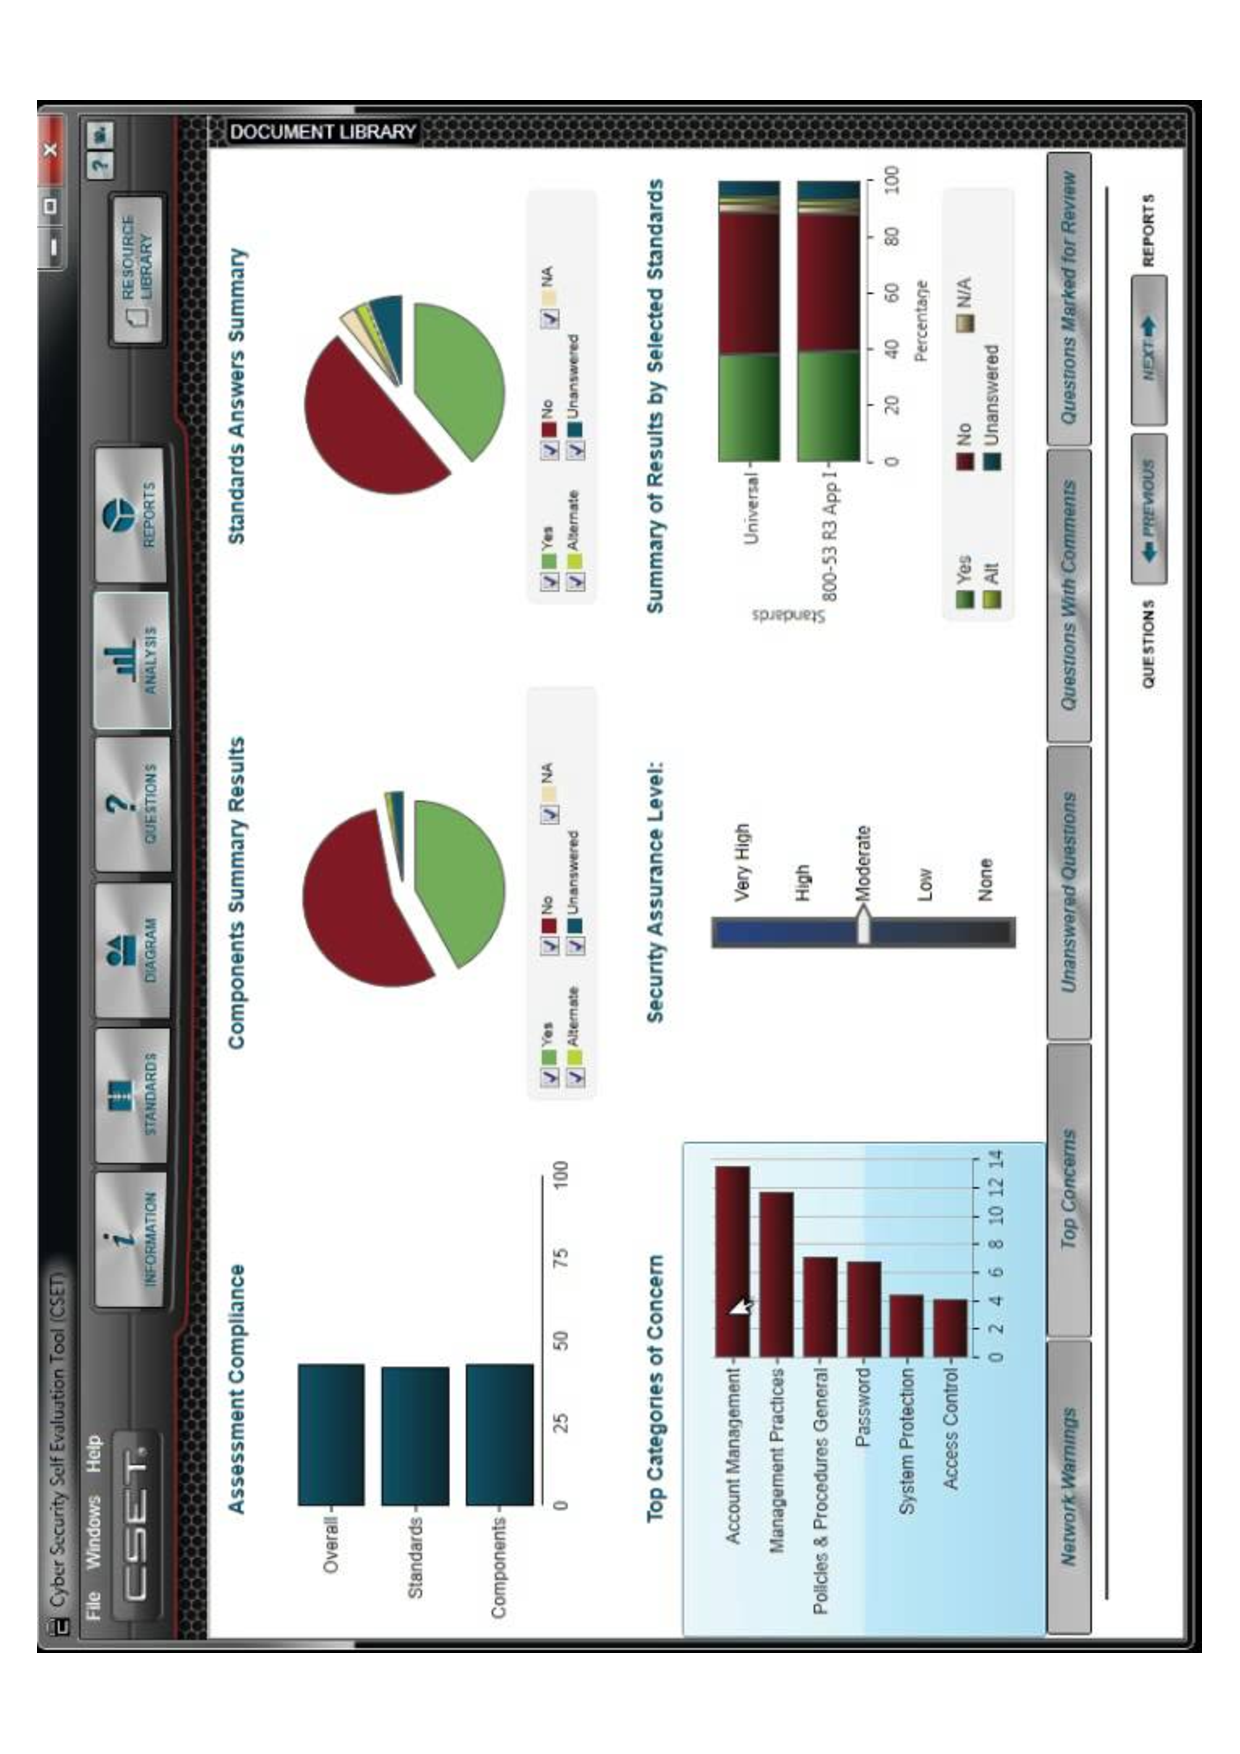
\includegraphics[height=8.5cm, angle=-90]{cset_figure}
\caption{Screenshot: CSET Report Overview \cite{cset_picture}}
\label{fig_elf}
\end{figure}

\subsection{TÜV-SÜD} \label{TUV}

\ac{TUV} is an international company specialized on ensuring the quality of medical devices and health care. The admission of medical products worldwide are shown in \ref{fig_twelve}. There are five product categories provided by TÜV-SÜD which will be explained in the following section.

First of all, TÜV-SÜD validates the market approval of medical devices\cite{tuev} and executes the certification process of qualified medical products. Based on in-depth knowledge and experience of key medical device markets around the globe, TÜV-SÜD has market access information for nearly every country. Particularly in the \ac{EU}, there are so-called 'EU Device Directives' which subdivide the regulation of different medical devices. TÜV-SÜD assumes the \ac{CE}-marking of medical devices, regulated in 93/42/EEC. \ac{AIMDD} have to be marked by CE, as described in 98/79/EEC. There also exist regulations for \ac{IVDD} which are specified in 98/79/EC.

%figure 12
\begin{figure}[!ht]
\centering
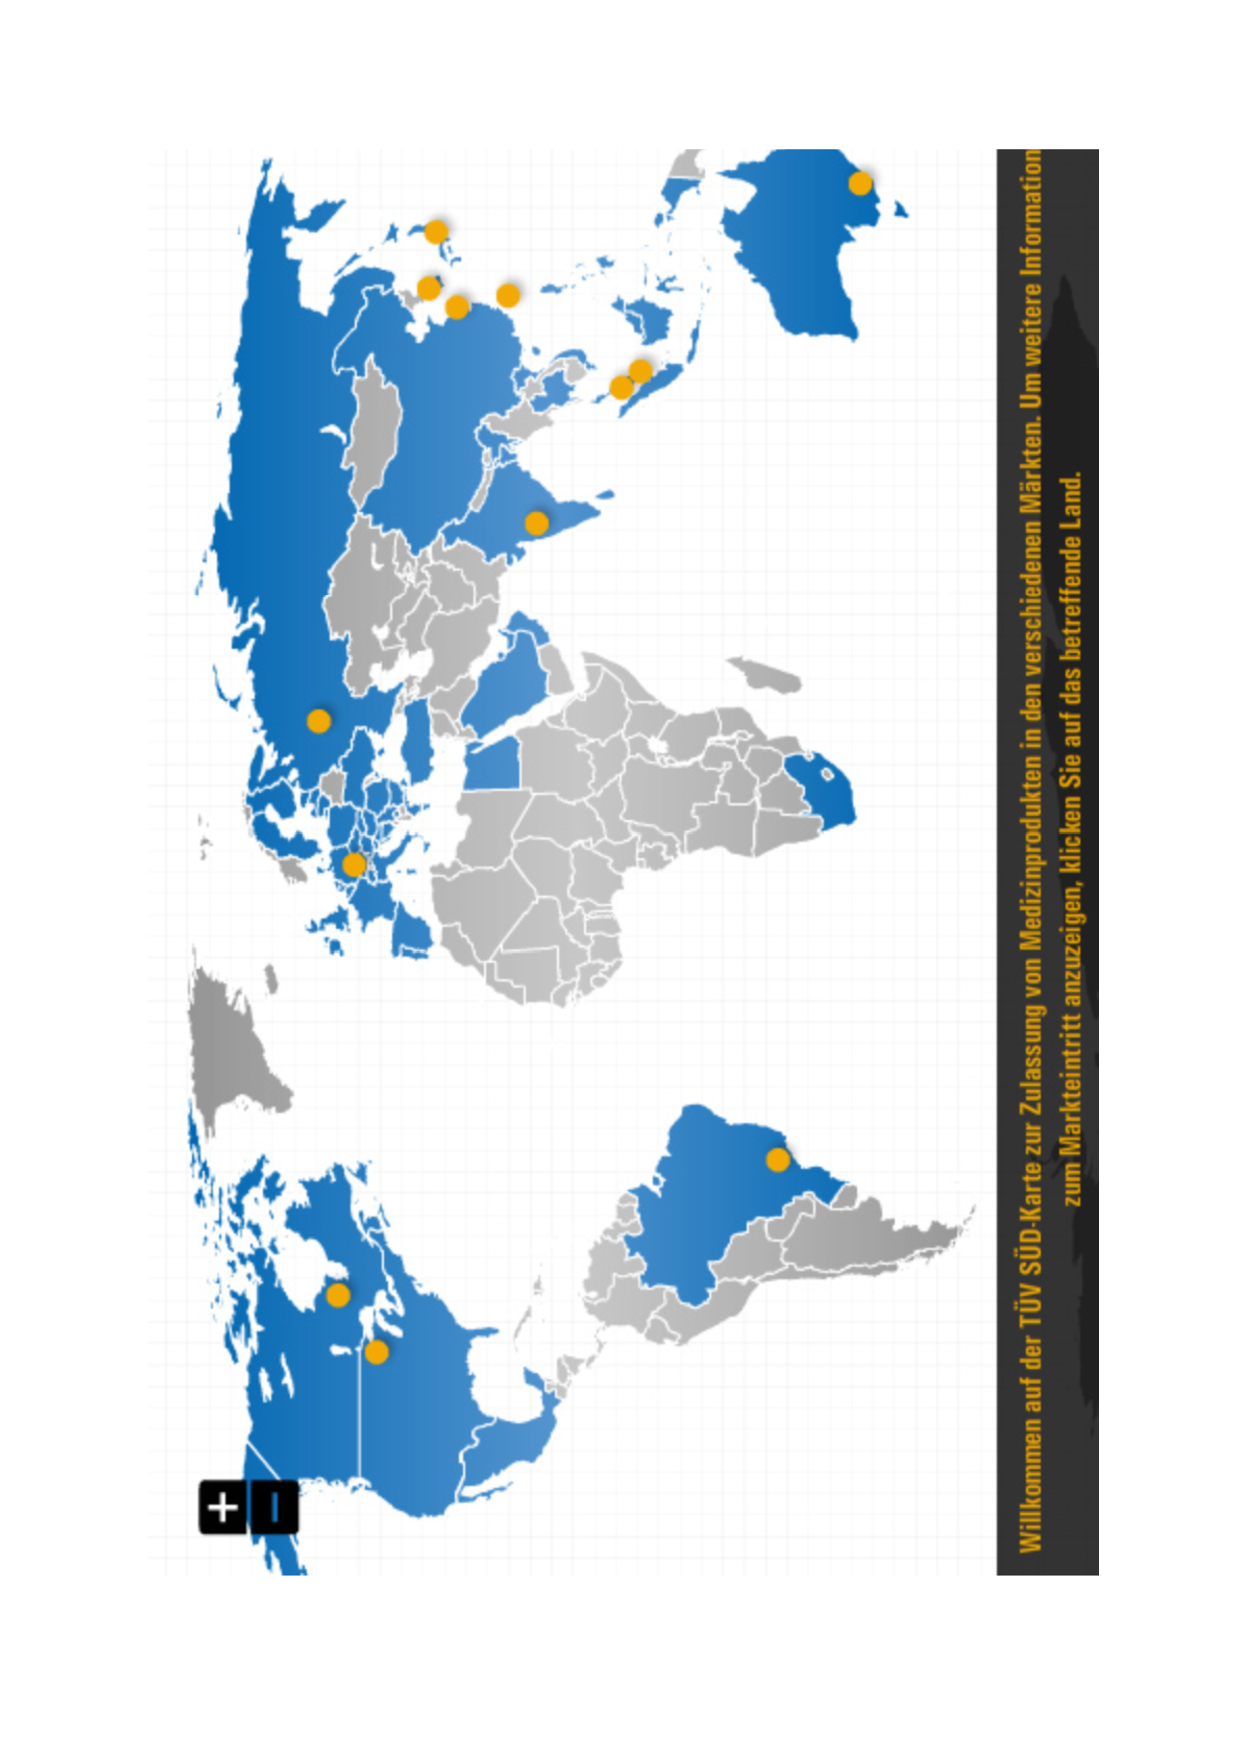
\includegraphics[height=8.5cm, angle=-90]{tuev_zulassung}
\caption{TÜV SÜD: Admission card of medical products \cite{tuev}}
\label{fig_twelve}
\end{figure}

Secondly, TÜV-SÜD performs tests and assessments which include the approval and testing of active and non-active medical devices. 

Thirdly, TÜV-SÜD provides quality management and quality control of medical devices. There are five important regulating \ac{ISO} standards: ISO 15378, 14971, 13485, 9001, 14001.

Fourthly, TÜV-SÜD provides clinical services for medical devices. These clinical services contain clinical data, clinical evaluation reports and clinical investigation plans for medical devices. 

After that, innovative medical devices are defined and assessed by TÜV-SÜD. These include devices with materials of animals origin, drug or service combination products. TÜV-SÜD provides  technical and regulatory due diligence support of the mentioned devices.

Last but not least, TÜV-SÜD offers support and upkeep to hospital and healthcare providers. Especially for dialysis, TÜV-SÜD certificates \ac{GDP} in hospitals. Additionally, the ISO 27001 which means 'Management System Certification' is executed by TÜV-SÜD.

\subsection{FDA} \label{FDA}

The mission of \ac{FDA} is to protect public health by 'ensuring safety, efficacy and security of human and veterinary drugs, biological products and medical devices' \cite{fda}. Especially food supply, cosmetics and products that emit radiation are tested for safety by the FDA. Furthermore, the FDA is responsible for regulating the manufactoring, marketing and distribution of tobacco products to protect public health and to reduce tobacco use by minors. 
In the health care sector, the FDA is responsible for advancing public health by helping to speed up innovations that make medical products more effective, safer and affordable for patients. Moreover, the FDA helps the public to get the accurate, science-based information they need to use medical devices. 

\ref{fig_thirteen} gives an impression of the procedure of approving a medical device, performed by the FDA. The approval process can be devided into five parts: 
\begin{itemize}
\item 'Concept and Design'
\item 'Pre-Clinical Engineering Development'
\item 'Clinical Trials: Proof of Concept Pivotal Trial'
\item 'FDA Review' 
\item 'Reimbursement Assignment'
\end{itemize}
The first two steps of the approval process are called 'Reimbursement Analysis' and lead to the examination of the \ac{IDE}. After the proof of concept, a FDA Submission is executed. In addition to the 'FDA Review', the device will be made accessible to patients.

Besides, the FDA plays a significant role in the U.S. Nation's counterterrorism capability. By ensuring the security of food supply and faster development of medical products, the FDA responds to deliberate and naturally emerging public health threats.

%figure 13
\begin{figure}[!ht]
\centering
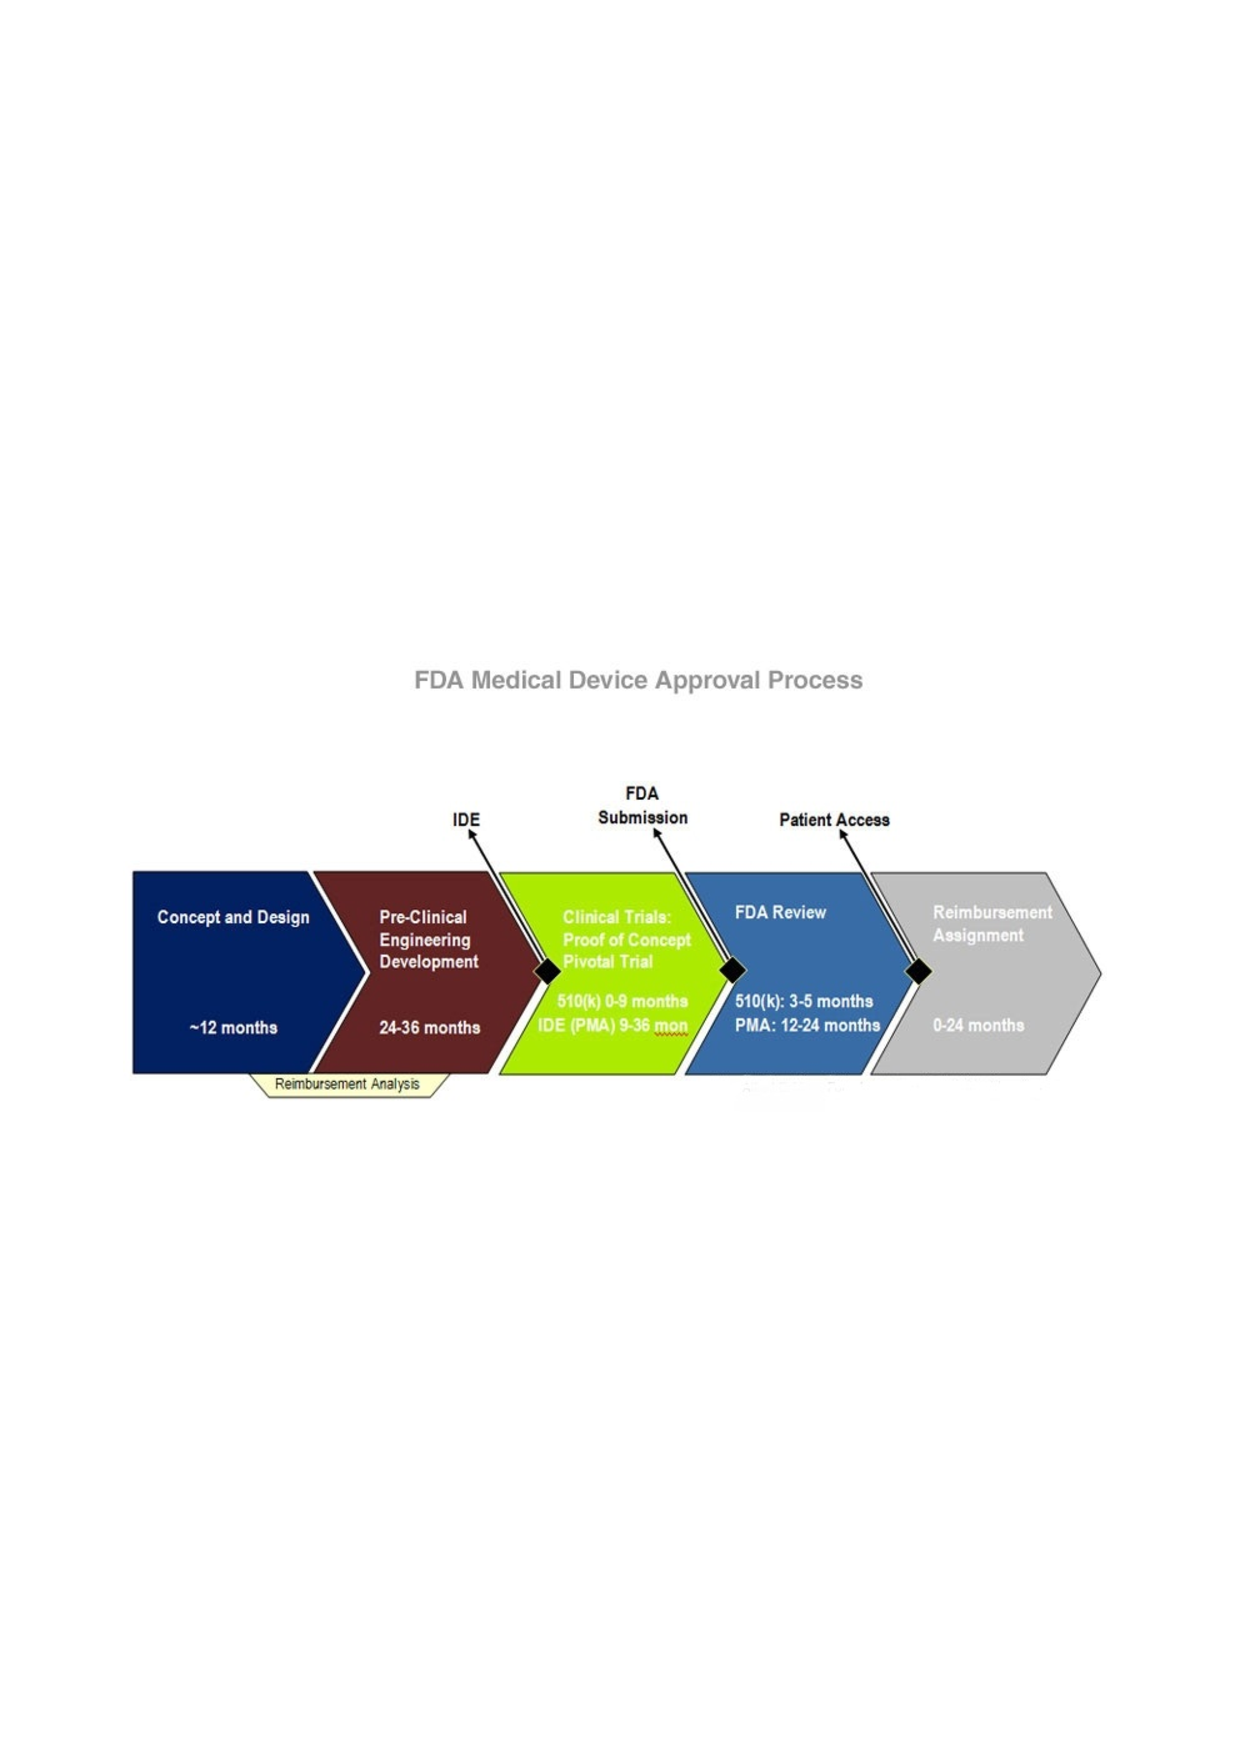
\includegraphics[width=8.5cm]{fda}
\caption{FDA Medical Device Approval Process \cite{fda_pic}}
\label{fig_thirteen}
\end{figure}

There are laws enforced by the FDA which will be explained in the next paragraph. In 1938, the 'Federal Food, Drug, Cosmetic Act' was passed and enforced by the FDA. 24 years later, in 1962, the 'Kefauver-Harris-Amendments' also known as 'Drug Efficacy Amendment' is an amendment to the 'Federal Food, Drug, and Cosmetic Act' of 1938. In 1976, 'Medical Device Amendments' were passed because of an incident, found out by the U.S. Senate. This incident included faulty medical devices and had caused 10,000 injuries, including 731 deaths \cite{fda}. The gist of the new law of 1976 was the safety and effectiveness to new medical devices.

As mentioned in the first paragraph, the FDA regulates foods, drugs, biologics, cosmetics, veterinary as well as tobacco products. In addition to that, medical devices and electronic products that give off radiation are also regulated by the FDA. Medical devices investigated by the FDA vary from simple items like bedpens to complex technologies such as heart pacemakers, dental devices and surgical implants or prosthestics.
Electronic products that give off radiation include microwave ovens, x-ray equipment, laser products, ultrasonic therapy equipment, mercury vapor lamps and sunlamps.    

\section{Outlook}

All in all, the subject medical devices should be clarified. There are several medical treatment solutions, which are applied after a diagnosed disease or are implanted in order to help the patient's body to work correctly, such as heart pacemakers. If the medical device was implanted, the talk is about \ac{IMD}. If these implantable medical devices are connected to an upper platform and communicate with each other, the network is called \ac{BAN}. One should know about the vulnerabilities of a BAN, e.g. about unsecure encryption of private patient data or about the misuse of the internal network in a hospital. Besides the encryption and secure transmission of personal data, the authentication and authorization process should be improved by using \ac{LDAP} and current technologies, like for example \ac{RFID} cards. In the end, there are several certification institutions in the USA and in Germany, which assess and control medical devices if they are compliant to the country's laws and restrictions. Whether a device will be published and deployed in practice, it has to be tested many times and should be compatible to international standards, like HL7 or DICOM.
Generally, everyone should be aware of the vulnerabilities and the consequences of attacks on medical devices, particularly for implantable medical devices. As an approach to solving this problem, security standards should be improved and neglected while producing medical devices and software. Furthermore every clinician should be aware of the access control via medical devices and has to assume his responsibility of a patients' life. But the last point is leading to another big issue which would go beyond the scope of this paper: Ethics and the protection of personal data privacy of patients.


%% --------------------------------------------------------------------

\section*{Abbreviations}
\addcontentsline{toc}{section}{Abbreviations}
\begin{acronym}[ICS-CERT]
\acro{MRT}{magnetic resonance tomograpy}
\acro{CT}{computer tomograpy}
\acro{FDA}{U.S. Food and  Drug Administration}
\acro{TUV}{Technischer Ueberwachungsverein}
\acro{ICS-CERT}{Industrial Control Systems Cyber Emergency Response Team} 
\acro{LAN}{Local Area Network} 
\acro{NIST}{National Institute of Standards and Technology}
\acro{WLAN}{Wireless Local Area Network} 
\acro{NFC}{Near Field Communication} 
\acro{IMD}{Implantable medical device} 
\acro{BAN}{Body Area Network} 
\acro{BIDMC}{Beth Israel Deaconess Medical Center}
\acro{NSF}{National Science Foundation}
\acro{ECG}{Electrocardiogram}
\acro{RF}{Radio Frequency}
\acro{RFID}{Radio Frequency Identification}
\acro{BCC}{Body-Coupled Communication}
\acro{OOB}{out-of-bound}
\acro{SDR}{Software defined radio}
\acro{LDAP}{Lightweight Directory Access Protocol}
\acro{VPN}{Virtual Private Network}
\acro{SSL}{Secure Sockets Layer}
\acro{TSL}{Transport Layer Security}
\acro{EU}{European Union}
\acro{CE}{Communauté Européenne}
\acro{IHE}{Integrating the Healthcare Enterprise}
\acro{ATNA}{Audit Trail and Node Authentication}
\acro{DICOM}{Digital Imaging and Communications in Medicine}
\acro{HL7}{Health Level Seven}
\acro{IVDD}{In Vitro Diagnostic Directives}
\acro{AIMDD}{Active Implantable Medical Device Directives}
\acro{ASTM}{American Society for Testing Materials}
\acro{HCMSS}{High Confidence Medical Device Software and System}
\acro{NCCIC}{National Cybersecurity and Communications Integration Center}
\acro{PIX}{Patient Identifier Cross-Referencing}
\acro{ISO}{International Organization for Standardization}
\acro{GDP}{Good Dialysis Practices}
\acro{SSO}{Single Sign-On}
\acro{XDS.b}{Cross-Enterprise Document Sharing}
\acro{IDE}{integrated development environment}
\acro{DES}{Data Encryption Standard}
\acro{3DES}{Triple Data Encryption Standard}
\acro{AES}{Advanced Encryption Standard}
\acro{ThaW}{Trustworthy Health and Wellness}
\end{acronym}

% Literaturverzeichnis
\addcontentsline{toc}{section}{References}
\printbibliography

\end{document}
